\chapter{Earthquake source generation}
\label{ch:source}

\section{Overview}

The EQRM conducts probabilistic seismic hazard analysis (PSHA) and
probabilistic seismic risk analysis (PSRA) using an event based
approach. This means that the ground motions (hazard) and loss
(risk) are computed for each event individually and the results
separately aggregated to form probabilistic estimates. The event
based approach differs from the traditional approach to PSHA which
integrate over all magnitude and distance combinations to attain
probability levels for exceeding a particular level of ground
motion in a pre-defined period of time. The traditional approach
is introduced by \citet{dr_Cornell68a} and summarised by
\citet{dr_McGuire90a}. A core component of any event based
analysis with the EQRM is the generation of a simulated
event\index{simulated event} (or earthquake) catalogue. The
generation of the earthquake catalogue relies upon an existing model for
the seismicity in the region. Typically the  model of seismicity comes
 from an interpretation of historical earthquakes,
 geology and neotectonics. The current version of the EQRM application requires a source model
that consists of a set of areal source zones (defined by a polygon) with associated
Gutenberg-Richter recurrence relationships and the option of including fault sources (defined by a plane) with associated 
Gutenberg-Richter or characteristic earthquake recurrence relationships \citet{dr_Schwartz84}. 

\emph{Areal source zones} typically capture the background seismicity in an area and are decribed by the acitivty rate within
each source zone through its Gutenberg-Richter \emph{a} and \emph{b} values. In event-based PSHA calculations, such as \typeself{E}{QR}{M},
synthetic ruptures will be generated stochastically throughout the areal source zone. However, a user may have sufficient information 
on the geometry and earthquake recurrence rates of a known fault and may want to place synthetic ruptures on the fault by defining a 
\emph{fault source}. In this instance, instead of placing the synthetic ruptures within the areal source zone, they will be placed 
on the known fault plane. \\

In addition, a novel technique has been developed to generate synthetic ruptures within a 3D volume that may represent seismotectonic 
features such as the intraplate environment of a subducting slab. Such events are often referred to as intraslab earthquakes and have been known
to generate larger and devastating earthquakes (e.g. 30 September 2009 Padang earthquake in Indonesia). \\

This chapter describes the process of creating an earthquake catalogue for probabilistic seismic hazard 
analysis and for defining an individual scenario event. The chapter is organised as follows. First the 
method of generating realistic ruptures in source zones and fault zones is discussed in Section \label{sec:source-EQgeom}. Second, the approach for 
determining recurrence rates is presented in Section \label{sec:source-EQrec}. Lastly, Section \label{sec:source-scen} 
describes scenario event generation.

\section{Creating an earthquake catalogue for probabilistic seismic hazard analysis}% a probabilistic seismic hazard analysis}
\label{sec:source-EQcat}

This section describes the method to generate a synthetic earthquake catalog of plausible events. The event catalog can be
created for events that are defined within an areal source or located on a known fault source. The recurrence relationship for the events
can be defined as a Gutenberg-Richter or Characteristic earthquake relationships.

A simulated event\index{simulated event} is represented by a plane
(or rupture) in 3D space that signifies the region where slip has
occurred. The geometry of a rupture plane is shown in
\Fref{fig:hrupture-3d}. The important parameters of a simulated
event\index{simulated event} are its location, geometry, magnitude
and activity (or likelihood of occurrence). The rupture trace is
the surface projection of the simulated event\index{simulated
event} along the direction of dip. The position and geometry of
the rupture trace is defined by its start $(r_s^{lat},r_s^{lon})$
and end $(r_e^{lat},r_e^{lon})$ points, its azimuth $r_{azi}$ and
its length $r_l$. The position and geometry of the rupture plane
are defined by its width $r_w$, dip $r_{dip}$ and the position of
its centre (or rupture centroid). The rupture centroid is defined
in cartesian coordinates $(r_x,r_y,r_z)$ in km using a local
coordinate system with origin at the rupture start point (see
\Fref{fig:hrupture-3d}). The orientation of the local coordinate
system is such that the $x-axis$ is oriented along the rupture
trace with positive direction pointing towards the rupture end
point, the $z-axis$ is pointing vertically downwards and the
$y-axis$ is oriented along the surface of the `earth' such that
the axes form a right handed triad. The vertical projection of the
rupture centroid is also described by its latitude $r_c^{lat}$ and
longitude $r_c^{lon}$. The event magnitude is represented as a
moment magnitude and is generated by the process described in
\sref{sec:magnitude_selection}. The activity (or likelihood of
occurrence) of the simulated event\index{simulated event} is
described by the event activity which represents the number of
times a given simulated event\index{simulated event} (conditional
on magnitude and position) occurs in one year (see
\sref{sec:magnitude_selection}).

\begin{figure}[htp]
\begin{center}
\begin{tabular}{ll}
(a) & (b) \\
% \psfrag{Fault Trace}{Rupture Trace} \psfrag{Dip}{$r_\theta$}
% \psfrag{Azimuth}{$r_\phi$}
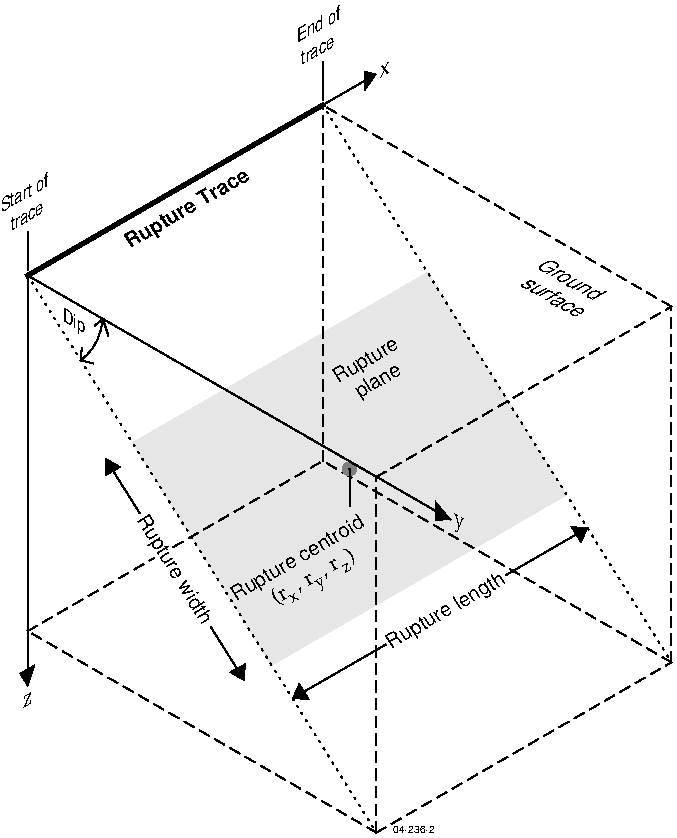
\includegraphics[width=0.49\textwidth]{diags/fig-hrupture-3d} &
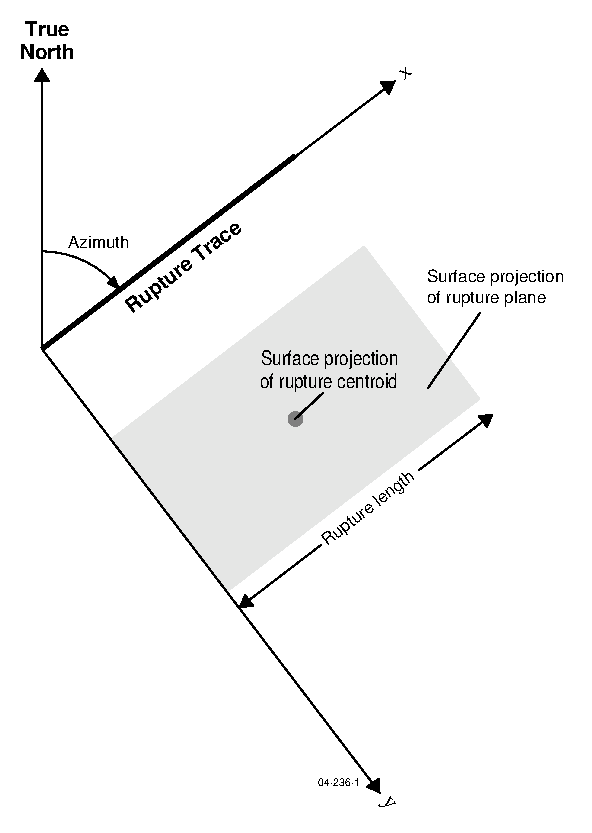
\includegraphics[width=0.41\textwidth]{diags/fig-hrupture-2d}
\end{tabular}
\end{center}
\caption{Orientation and dimension of the rupture plane in (a) 3D
and (b) 2D vertical projection to ground surface.}
\label{fig:hrupture-3d}
\end{figure}




\begin{table}
\centering \caption{Columns in \typevarcaption{ev}{nt}{db}. Note
that some of the columns are not defined until after
\typefunccaption{fuse}{4}{\_hzd} is run (see
\sref{source:spawning}).}
 \label{tab:evntdb-columns}
\vspace{0.8em}
\begin{tabular}{r|p{0.85\textwidth}}
\hline
column & description \\
\hline
1 & an integer corresponding to the generation source zone from which this event was generated \\
2 & $r_s^{lat}$ - latitude of rupture trace start point (decimal degrees)\\
3 & $r_s^{lon}$ - longitude of rupture trace start point (decimal degrees)\\
4 & $r_e^{lat}$ - latitude of rupture trace end point (decimal degrees)\\
5 & $r_e^{lon}$ - longitude of rupture trace end point (decimal degrees)\\
6 & $r_\phi$ - azimuth of rupture trace (decimal degrees from True North)\\
7 & $r_{dip}$ - dip of rupture plane (0 $<$ decimal degrees $<$ 90 from the surface) \\
8 & $A_{min}$ - number of earthquakes of magnitude $m_{min}$ or greater per year\\
9 & integer pointer to attenuation model for use with the synthetic earthquake.\\
10 to 18 & place holder (currently not used) \\
19 & $w_e$ - weight derived from event spawning  \\
20 & $r_\nu$ - event activity (the number of magnitude $r_m$ earthquakes expected per year scaled to the number being simulated) \\
21 & $r_m$ - event magnitude (moment magnitude)\\
22 & $r_\varepsilon$ - source epsilon from event spawning\\
23 & $r_c^{lat}$ - latitude of event centroid (decimal degrees) \\
24 & $r_c^{lon}$ - longitude of event centroid (decimal degrees) \\
25 & $r_z$ - event centroid depth z (km from ground surface) \\
26 & $r_x$ - event centroid x (km along rupture trace from the
start of trace) \\
27 & $r_y$ - event centroid y (km perpendicular from trace in
direction of
dip) \\
28 & $r_l$ - length of rupture (km) \\
29 & $r_w$ - width of rupture (km measured along dip) \\
30 & a unique integer for each synthetic earthquake in the generation zone (polygon). Note that the integer count begins again for each generation zone. \\
31 & place holder (currently not used) \\
\hline
\end{tabular}
\end{table}


\subsection{Simulated events and virtual fault\index{virtual fault}s}

The terms simulated event\index{simulated event}, simulated
earthquake\index{simulated earthquake} and simulated
rupture\index{simulated rupture} are congruent and will be used
interchangeably throughout this document. Sometimes the adjective
`simulated' will be omitted for brevity. An adjective `actual'
will be used in place of `simulated' to refer to a historic
earthquake (i.e. one that has actually occurred rather than one
that is simulated).

A virtual fault\index{virtual fault} refers to a plane in 3D space upon which an event can
occur.  The virtual fault can be located in within an areal source or defined by a known fault. 
The \typeself{E}{QR}{M} works by first creating a virtual fault\index{virtual fault}, either within an
areal source zone, or by a user defined know fault. The rupture is then placed 
on the virtual fault\index{virtual fault} (the
rupture is not allowed to exceed the bounds of the virtual
fault\index{virtual fault}). The introduction of a virtual
fault\index{virtual fault} is the mechanism by which the
\typeself{E}{QR}{M} application constrains the location and extent
of each rupture. The depth to the top of a virtual
fault\index{virtual fault} is defined as the depth to the
seismogenic region $f_z$ (see
\tref{tab:site-loc-par-sourcezones}). Other geometrical parameters
of virtual fault\index{virtual fault}s include the width $f_w$ and
length $f_l$. 


\subsection{Location of synthetic earthquakes in areal sources}
\label{sec:rup-location}

The location of each event is assigned randomly within an areal source zone 
and on a fault source. 
This assignment is done in such a way that the event has
an equal probability of being located anywhere in the `generation
polygon' or on the fault. 

The first phase of locating the events involves positioning the
centre point of each rupture trace ($r_c^{lat}$,$r_c^{lon}$). A
rectangular box is generated over the top of the source zone polygon. The
box is bounded by the minimum and maximum latitude and the
minimum and maximum longitude of the source zone itself. 

% Need to change this to have no underlying grid. 
\begin{figure}
\begin{center}
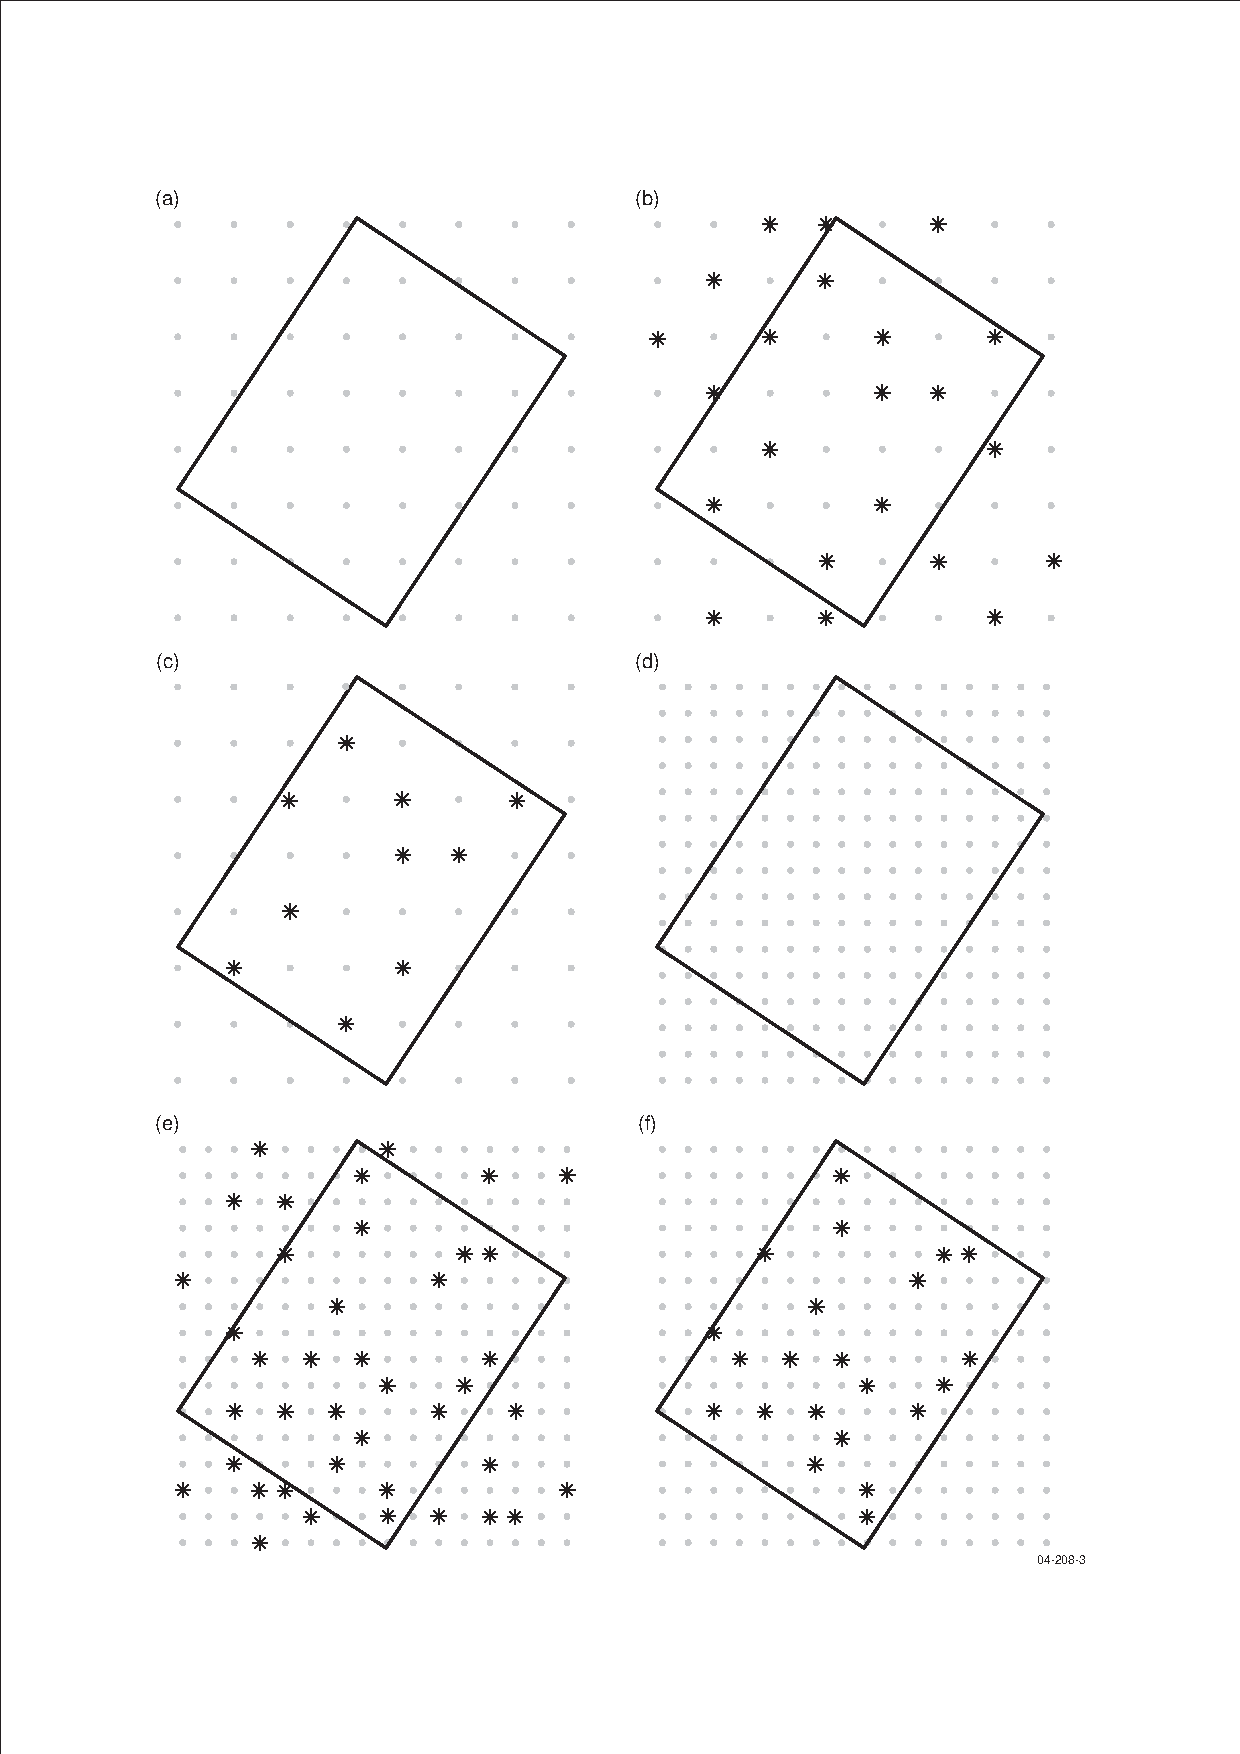
\includegraphics[width=0.9\textwidth]{fig-hsource-trace-starts}
\end{center}
\caption{Random selection of rupture centroids for a
rectangular `generation polygon'. (a) to (c) illustrate the first
iteration and (d) to (f) the second iteration after contraction of
the grid spacing.} \label{fig:source-trace-starts}
\end{figure}

The rupture centroid of each event is then randomly placed within the box 
using a discrete uniform probability density function
(\fref{fig:source-trace-starts}b). The event is the checked to identify whether 
it falls within the source polygon or not. Events that fall within the source polygon 
are kept and those that lie outside it are discarded. 

The second phase of locating events involves positioning the start and end
point of the rupture trace. Assume for the moment that both the
length and azimuth of the rupture trace are already known (see
\sref{sec:dim-rupture} and \sref{sec:az-dip-rupture} respectively
for a description of how these are computed). It is then a trivial
process to compute the start and end of the rupture trace
$(r_s^{lat},r_s^{lon} and r_e^{lat},r_e^{lon})$. It is important to note that the \typeself{E}{QR}{M} will allow the 
start or end points of the rupture trace to lie outside of the source polygon 
providing the rupture centroid is located within the polygon. The source zone polygon 
is only used to constrain the rupture centroid ($r_c^{lat},r_c^{lon}$).

\subsection{Location of events on fault sources}

As discussed earlier in this chapter, fault sources in the \typeself{E}{QR}{M} can represent three different styles of faulting:

\begin{itemize}
\item Crustal faults
\item Subduction interface faults
\item Intraslab faults in the subducting slab
\end{itemize}

The method for placing synthetic ruptures on crustal faults and subduction interface faults is the same, but intraslab faults required a 
different approach. \\

\subsubsection{Crustal Faults and Subduction Interface Faults}
Assuming again that we have already defined the length and width of the rupture plane, we then solve to find the location of the rupture
trace along the predefined fault trace by:

\begin{equation} \label{eq:ds}
D_s = (f_l - r_l) \times \mathtt{X}
\end{equation}

where $\mathtt{X}$ is a random variable between 0$\rightarrow$1. Following this step the new start and end of the rupture trace can be 
obtained using the rupture length, azimuth of the fault. \\

We now use $D_s$ from equation \ref{eq:ds}, and the precalculated rupture length and fault azimuth to calculate the 
new longitude and latitude of the start and end of the rupture trace (\ref{fig:traces}). 

% \begin{figure}[htp]
% \centerline{\includegraphics[width=6cm]
% {faulttrace.png}}
% \caption{A plan view of the fault trace and rupture trace defined by its start and end coordinates.}
% \label{fig:traces}
% \end{figure}

We now follow a similar process (to equation \ref{ds}) to determine the depth of the rupture centroid. Since we 
already have the fault width we can randomly assign the depth of the rupture centre while making sure the rupture 
plane does not extend beyond the top and bottom of the fault plane defined in the source file (\ref{fig:rzrange}). 

% \begin{figure}[htp]
% \centerline{\includegraphics[width=12cm]
% {depthrange.png}}
% \caption{A schematic diagram of how we define the depth range of the rupture centroid.}
% \label{fig:rzrange}
% \end{figure}

We first find the depth range which the rupture centroid can lie within [$r_z^{min}, r_z^{max}$] such that 
the rupture plane does not extend above or below the bounds of the seismogenic zone [$f_z^{top}, f_z^{bot}$]:

\begin{subequations} \label{drange}
\begin{align}
r_z^{min} & = \mbox{minimum depth of rupture centroid}  \\
r_z^{max} & = \mbox{maximum depth of rupture centroid}   \\
r_z^{min} & = r_z^{top} + 0.5r_w  \times sin(r_\theta  \times \mbox{rad})    \\
r_z^{max} & = r_z^{bot} - 0.5r_w  \times sin(r_\theta \times \mbox{rad})  
\end{align}
\end{subequations}

where $f_\theta = r_\theta$. Note that for intrapate ruptures which will be discussed later $f_\theta \ne r_\theta$. 
We can now randomly assign the rupture centroid depth using a uniform distribution between $r_z^{min}$ and $r_z^{max}$ 
using the \texttt{numpy} package in \texttt{python}:

\begin{equation} \label{eq:rand}
	r_z = ( r_z^{max}-r_z^{min} ) \times  \mathtt{X} +   r_z^{min}
\end{equation}

where $\mathtt{X}$ is a random varaible from 0$\rightarrow$1. The local x and y coordinates ($r_x$ and $r_y$) of the rupture 
centroid can be calculated by the employing the same equations as for the source zones:

\begin{equation}
r_y = r_z  \frac{cos(f_\theta  \times rad)}{sin(f_\theta  \times rad)}
\end{equation}

\begin{equation}
r_x = \frac{r_l}{2}
\end{equation}

Where the rupture centroid location in local coordinates ($r_x$, $r_y$) can be converted to longitude and latitude ($r_c^{lon}$, $r_c^{lat}$).

\subsubsection{Intraslab Faults}

The concept of creating realistic ruptures that represent events in a subducting slab is achieved by considering these events as 
out of plane ruptures. The subducting slab is defined as a 3D plane from which rupture planes extend out from at angles defined by
the user (FIGURE PLOT). For this functionality and out of dip value must be defined ($\delta_\theta$). 
This parameter defines the angle between the dipping fault and the rupture plane (figure \ref{fig:intraslabGeom}). If the rupture 
plane is parallel to the fault plane this value will be zero. If the rupture plane is it an angle to the dipping plane then it 
will be non-zero. When handling a non-zero $\delta_\theta$ we also need to consider another parameter, $\Delta_\theta$, which 
defines the range of dips we will sample across to obtain the rupture dip ($r_\theta$, figure \ref{fig:intraslabGeom}).
We first take a uniform sample from the range [$\delta_\theta - \Delta_\theta, \delta_\theta + \Delta_\theta$]  to determine 
the out of plane angle ($\omega$) and the dip of the rupture plane ($r_\theta$) :


\begin{equation}
\omega = 2\Delta_\theta  \times \mathtt{numpy.random.random\_sample()} + \delta_\theta - \Delta_\theta
\end{equation}

\begin{equation}
r_\theta = \omega + f_\theta
\end{equation}

When dealing with out of plane ruptures we need to consider two cases:
\begin{itemize} 
\item $0 \leq r_\theta \leq 90:$ \\ In this instance the rupture plane will dip in the same direction as the fault plane and we need to project the new rupture plane to the surface to define the surface trace of the rupture.
\item $90 <  r_\theta \leq 180:$ \\ In this case the rupture plane dips in the opposite direction to the fault plane and the local coordinate system must be transformed because the plane is no longer dipping to the right handside of the trace when looking from the start to the end of the trace. We must project the new rupture plane to the surface and then redefine the start and end locations of the rupture trace. This is because we always work in a right-handed local coordinate system with the rupture plane dipping to the right of the trace when looking along the trace from the start location to the end locatio (figure \ref{fig:intraslabGeom}).  
\item $180 < r_\theta \leq f_\theta + \omega :$ \\ In this case the rupture plane dips in the same direction of the fault plane, but the rupture trace is projected in the negative y direction of the local coordinate system. 
\end{itemize}
\begin{figure}[htp]
\centerline{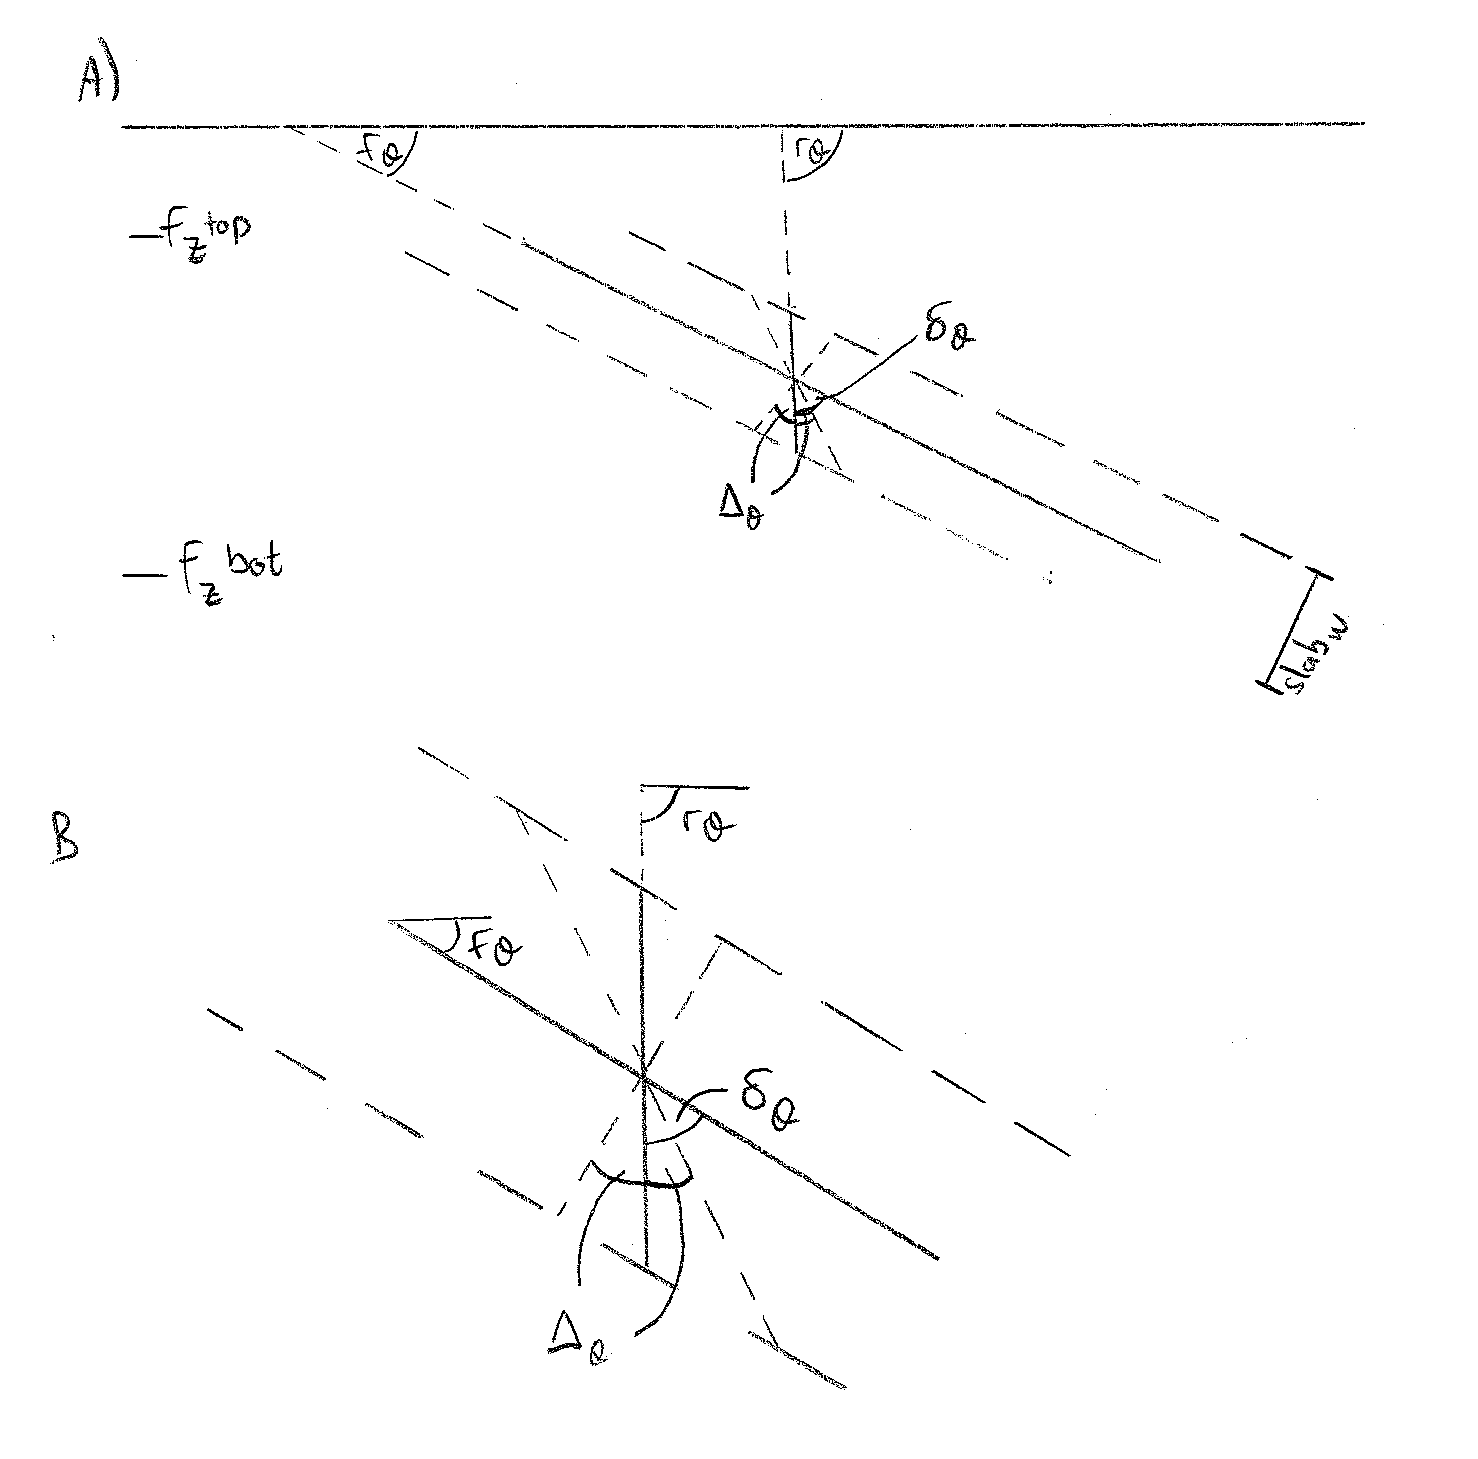
\includegraphics[width=16cm]
{geomoutplane}}
\caption{A schematic diagram of the geometry of out of plane ruptures. Panel A shows the rupture plane dipping out of the fault plane that defines the dipping slab. Panel B is a zoom in of the angles that define the rupture plane geometry. The user defines the fault dip ($f_\theta$), which in this case represents the direction of the downgoing slab, and the out of plane dip ($\delta_\theta$) and a sampling range ($\Delta_\theta$) over which the EQRM will uniformly distribute the rupture plane. }
\label{fig:intraslabGeom}
\end{figure}



%%%%%
\subsection{Case if  $0 \leq r_\theta \leq 90$} \label{sec:0to90}
%%%%%

We follow a similar approach to that in section \ref{sec:faultplane} where we first define the rupture plane dimensions (area $r_A$, width $r_w$ and length $r_l$). We force the rupture dimensions to fall within the length of the fault, but this time we must also not allow it to extend outside of the width of the dipping slab ($S_w$) defined in the source file. As shown in figure \ref{fig:deltaeq} we can find the maximum width of the rupture plane ($r_w^{max}$) from:

\begin{equation}\label{rwmax}
r_w^{max} = 
\begin{cases}
 \frac{ S_w }{sin (\omega \times rad)}		& \quad \mbox{if $\omega$ $<$ 90} \\
S_w							& \quad \mbox{if $\omega$ $=$ 90} \\
 \frac{ S_w }{sin ((180 - \omega ) \times rad)}	& \quad \mbox{if $\omega$ $>$ 90} \\
\end{cases}
\end{equation}

% old way
%\begin{equation} 
%r_w^{max} = \frac{ slab_w }{sin ((r_\theta - f_\theta) \times rad)}
%\end{equation}

\begin{figure}[htp]
\centerline{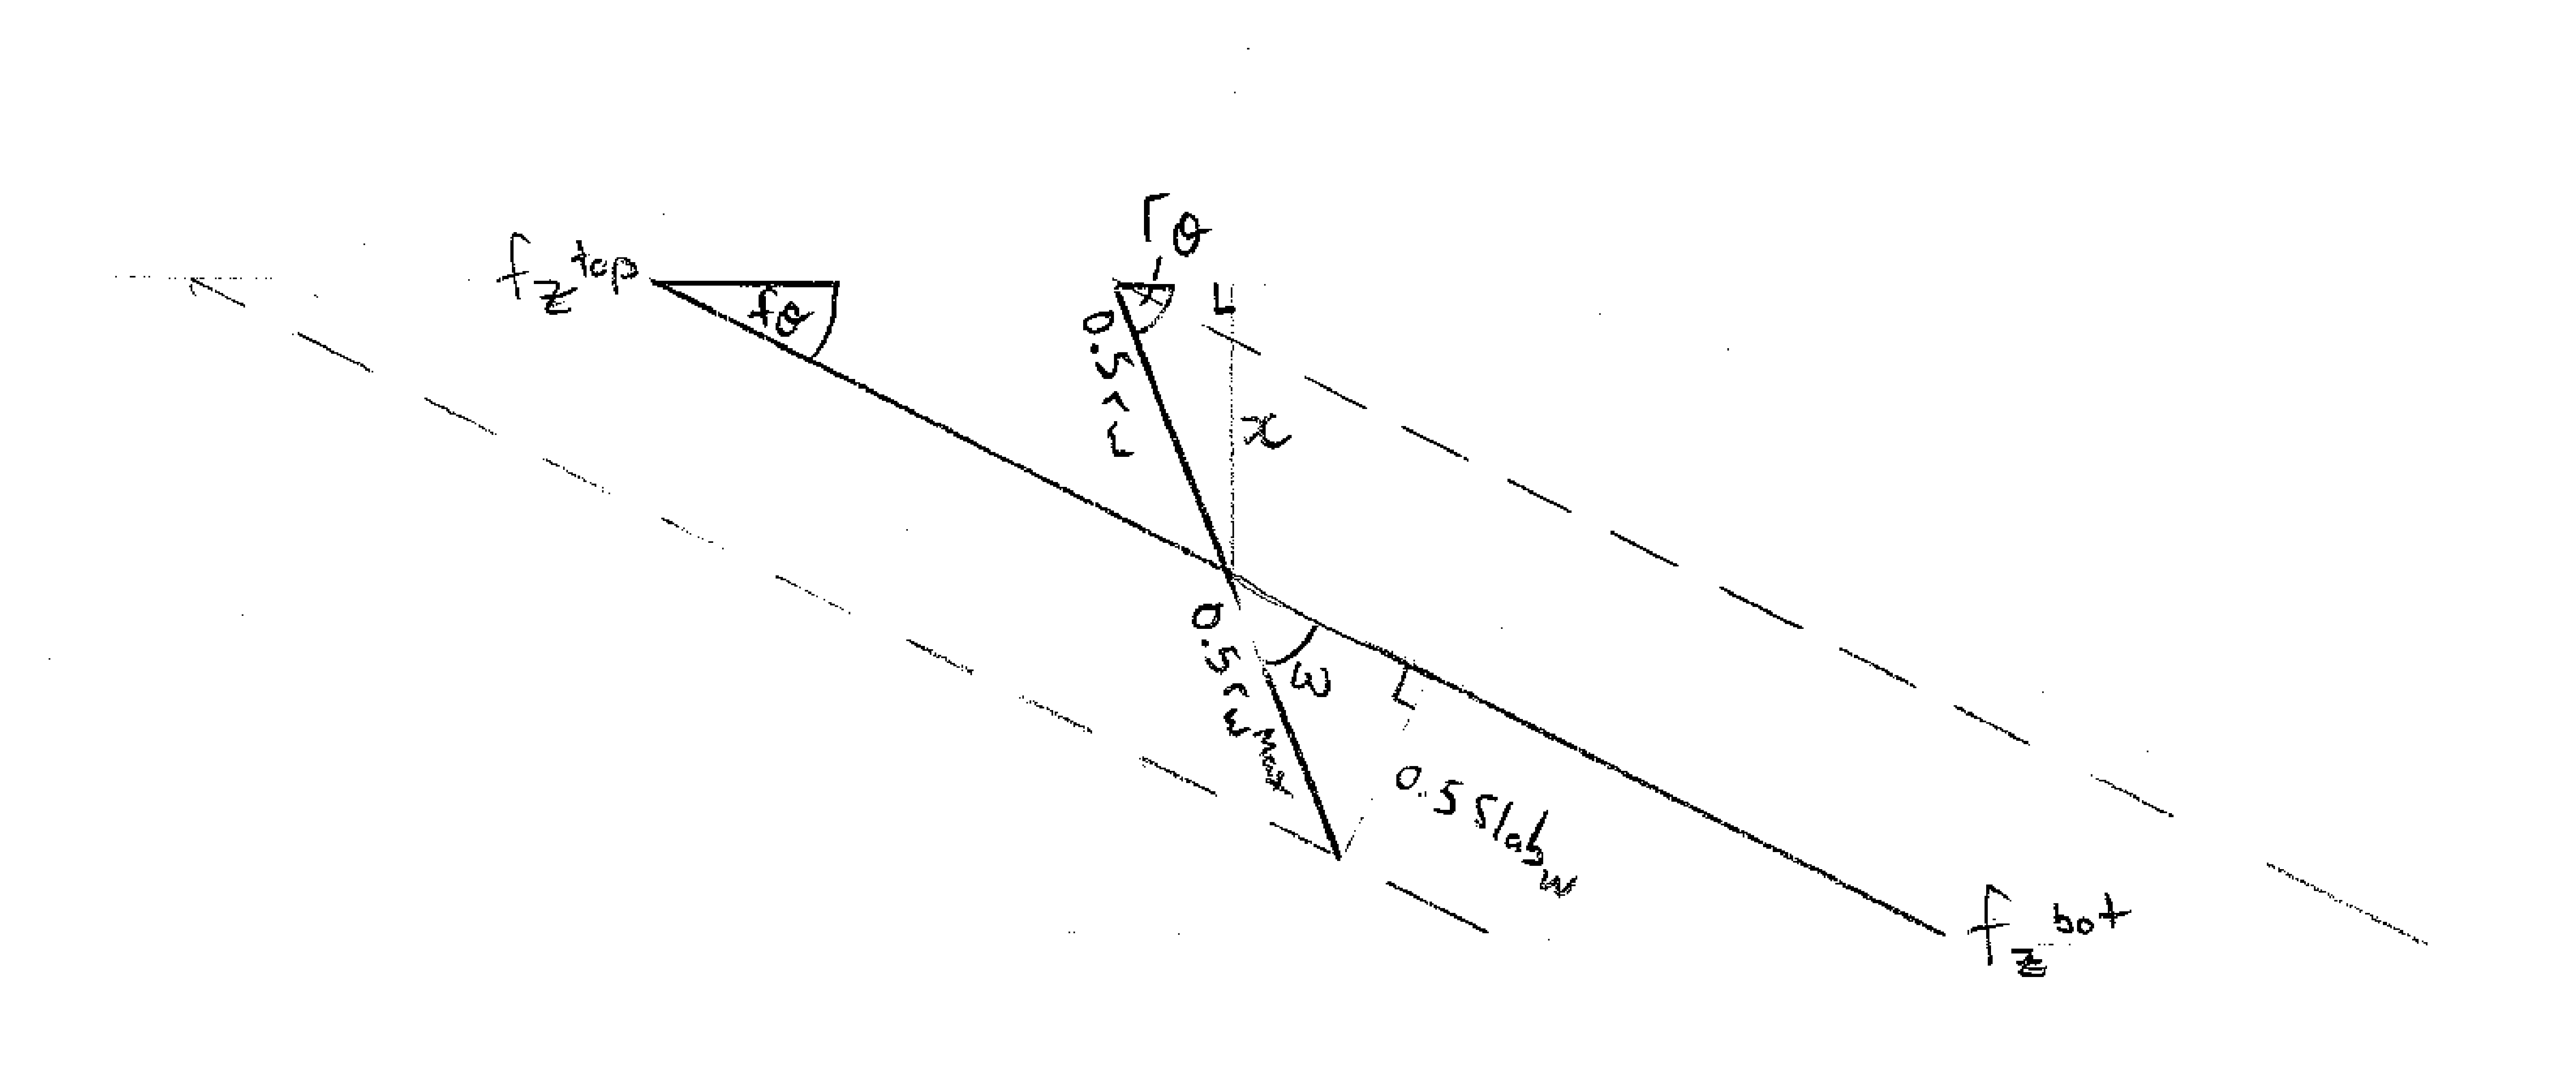
\includegraphics[width=12cm]
{geomwidth}}
\caption{The geometry of determining the maximum rupture width ($r_w^{max}$) shown in the lower trigonometric geometry and the $r_z^{min}$ and $r_z^{max}$ shown in the upper part and equation \ref{drange2}.}
\label{fig:deltaeq}
\end{figure}

We use equations \ref{ra} and \ref{rw} to calculate the rupture area ($r_A$) and rupture width ($r_w^{WC}$) from the Wells and Coppersmith, 1994 scaling laws. But for out of plane ruptures we must limit the rupture width ($r_w$) not to the fault width as is the case of on plane ruptures, but to not extend beyond the slab boundary. Therefore we use a slightly modified version of equation \ref{eq:rw} to solve for the rupture width:

\begin{equation} \label{rw090}
r_w = \mathbf{min}\{ r_w^{WC}, r_w^{max}\}
\end{equation}

now we can calculate the rupture length ($r_l$), making sure it does not extend beyond the fault length ($f_l$) from:

\begin{equation}
r_l = \mathbf{min}\left\{\frac{r_A}{r_w}, f_l\right\}
\end{equation}

We use equation \ref{ds} to calculate $D_s$, the distance (km) along the fault trace for the start of rupture trace and equations \ref{eq:newrs} and \ref{eq:newre} to find the position of the start and end of the rupture trace. Note that we use new notation to describe the location of the start and end of the rupture trace along the fault trace ($\hat{r}_e^{lon}$, $\hat{r}_e^{lat}$, $\hat{r}_e^{lon}$, $\hat{r}_e^{lat}$) this is because soon we will need to define the new location of the rupture trace ($r_s^{lon}$, $r_s^{lat}$ and $r_e^{lon}$, $r_e^{lat}$):

\begin{equation}\label{eq:newrs2}
\hat{r}_s^{lon},\hat{r}_s^{lat} =\mathtt{get\_new\_ll}(f_s^{lon}, f_s^{lat}, f_\phi, D_s)
\end{equation}

\begin{equation}\label{eq:newre2}
\hat{r}_e^{lon}, \hat{r}_e^{lat} =\mathtt{get\_new\_ll}(\hat{r}_s^{lon}, \hat{r}_s^{lat}, f_\phi, r_l)
\end{equation}

Next we need to redefine the depth range of the random depth allocation similar to that of equation \ref{drange} to make sure the rupture trace does not go above or below the seismogenic zone of the fault. This is slightly different to equation \ref{drange} because the rupture plane is now dipping out of the fault plane (figure \ref{fig:deltaeq}).

\begin{subequations} \label{drange2}
\begin{align}
r_z^{min} & = \mbox{minimum depth of rupture centroid}  \\
r_z^{max} & = \mbox{maximum depth of rupture centroid}  \\
r_z^{min} & = f_z^{top} + 0.5r_w  \times sin(r_\theta  \times \mbox{rad})    \\
r_z^{max} & = f_z^{bot} - 0.5r_w  \times sin(r_\theta  \times \mbox{rad})  
\end{align}
\end{subequations}

Using equation \ref{eq:rand} we can now randomly assign the rupture centroid depth using a uniform distribution between $r_z^{min}$ and $r_z^{max}$ using the \texttt{numpy} package in \texttt{python}:
\begin{equation}
r_z = ( r_z^{max}-r_z^{min} ) \times  \mathtt{numpy.random.random\_sample()} +   r_z^{min}
\end{equation}

We now need to project the rupture trace to the surface to obtain the surface trace, and then the rupture centroid. 
We begin by finding the location of the rupture centroid referenced to the start position of the original fault plane:
\begin{equation}\label{eq:ry}
\hat{r}_y = r_z  \frac{cos(f_\theta  \times rad)}{sin(f_\theta \times rad)}
\end{equation}

and then:
\begin{equation}
\hat{r}_x = \frac{r_l}{2}
\end{equation}

We now need to determine the start and end position of the surface trace for the rupture plane. We do this by first 
finding the location referenced to the start location of the rupture ($r_s^{lon}$, $r_s^{lat}$) along the fault 
plane (equations \ref{eq:newrs} and \ref{eq:newre}) then convert to latitude and longitude.

\begin{equation}\label{eq:rsx}
\hat{r}_s^{x} = 0
\end{equation}

and now we substitute the dip of the rupture plane ($r_\theta$) into equation \ref{eq:ry}

\begin{equation}
\hat{r}_s^{y} = \hat{r}_y - r_z  \frac{cos(r_\theta \times rad)}{sin(r_\theta \times rad)}
\end{equation}

\begin{equation}\label{eq:rex}
\hat{r}_e^{x} = r_l
\end{equation}

\begin{equation}\label{eq:rey}
\hat{r}_e^{y} = \hat{r}_s^{y}
\end{equation}

Now we can calculate the longitude and latitude for the start and end of the rupture trace.


Now all that is left is to redefine the location of the rupture centroid in local x and y coordinates relative to the origin 
($r_s^{lon}$,$ r_s^{lat}$) of the new local coordinate system:
\begin{equation}\label{eq:rx}
r_x = 0.5 r_l
\end{equation}

\begin{equation}
r_y = r_z  \frac{cos(r_\theta \times rad)}{sin(r_\theta \times rad)}
\end{equation}

and then transform this into longitude and latitude:
\begin{equation}\label{eq:rcll}
r_c^{lon}, r_c^{lat} = \mathtt{azimuthal\_orthographic\_xy\_to\_ll}(r_x, r_y,r_s^{lon},r_s^{lat},f_\phi,\mbox{R}=6367.0) .
\end{equation}

Note that $r_z = \hat{r}_z$.

%%%%%
\subsection{Case if $90 <  r_\theta \leq 180$} \label{sec:90t180}
%%%%%

In this instance the rupture plane is dipping in the opposite direction to the fault plane. Recall that if we look along 
the rupture trace the plane always dips to the right hand side, therefore in the case here of rupture plane the dips 
opposite to the project of the surface trace we need to re-project the rupture plane to the surface then swap the 
start and end coordinates. 


% $90 <  r_\theta \leq 180$

After calculating $r_w^{max}$ from equation \ref{rwmax} we then must obtain $r_\theta$such that it lies between 5 and 90:

\begin{equation}
r_\theta = \mathbf{max} \{ 180 - f_\theta + \omega, 5 \} .
\end{equation}


%\begin{equation}
%r_w^{max} = \frac{ slab_w }{sin ((180 - (r_\theta - f_\theta)) \times rad)}
%\end{equation}

\begin{figure}[htp]
\centerline{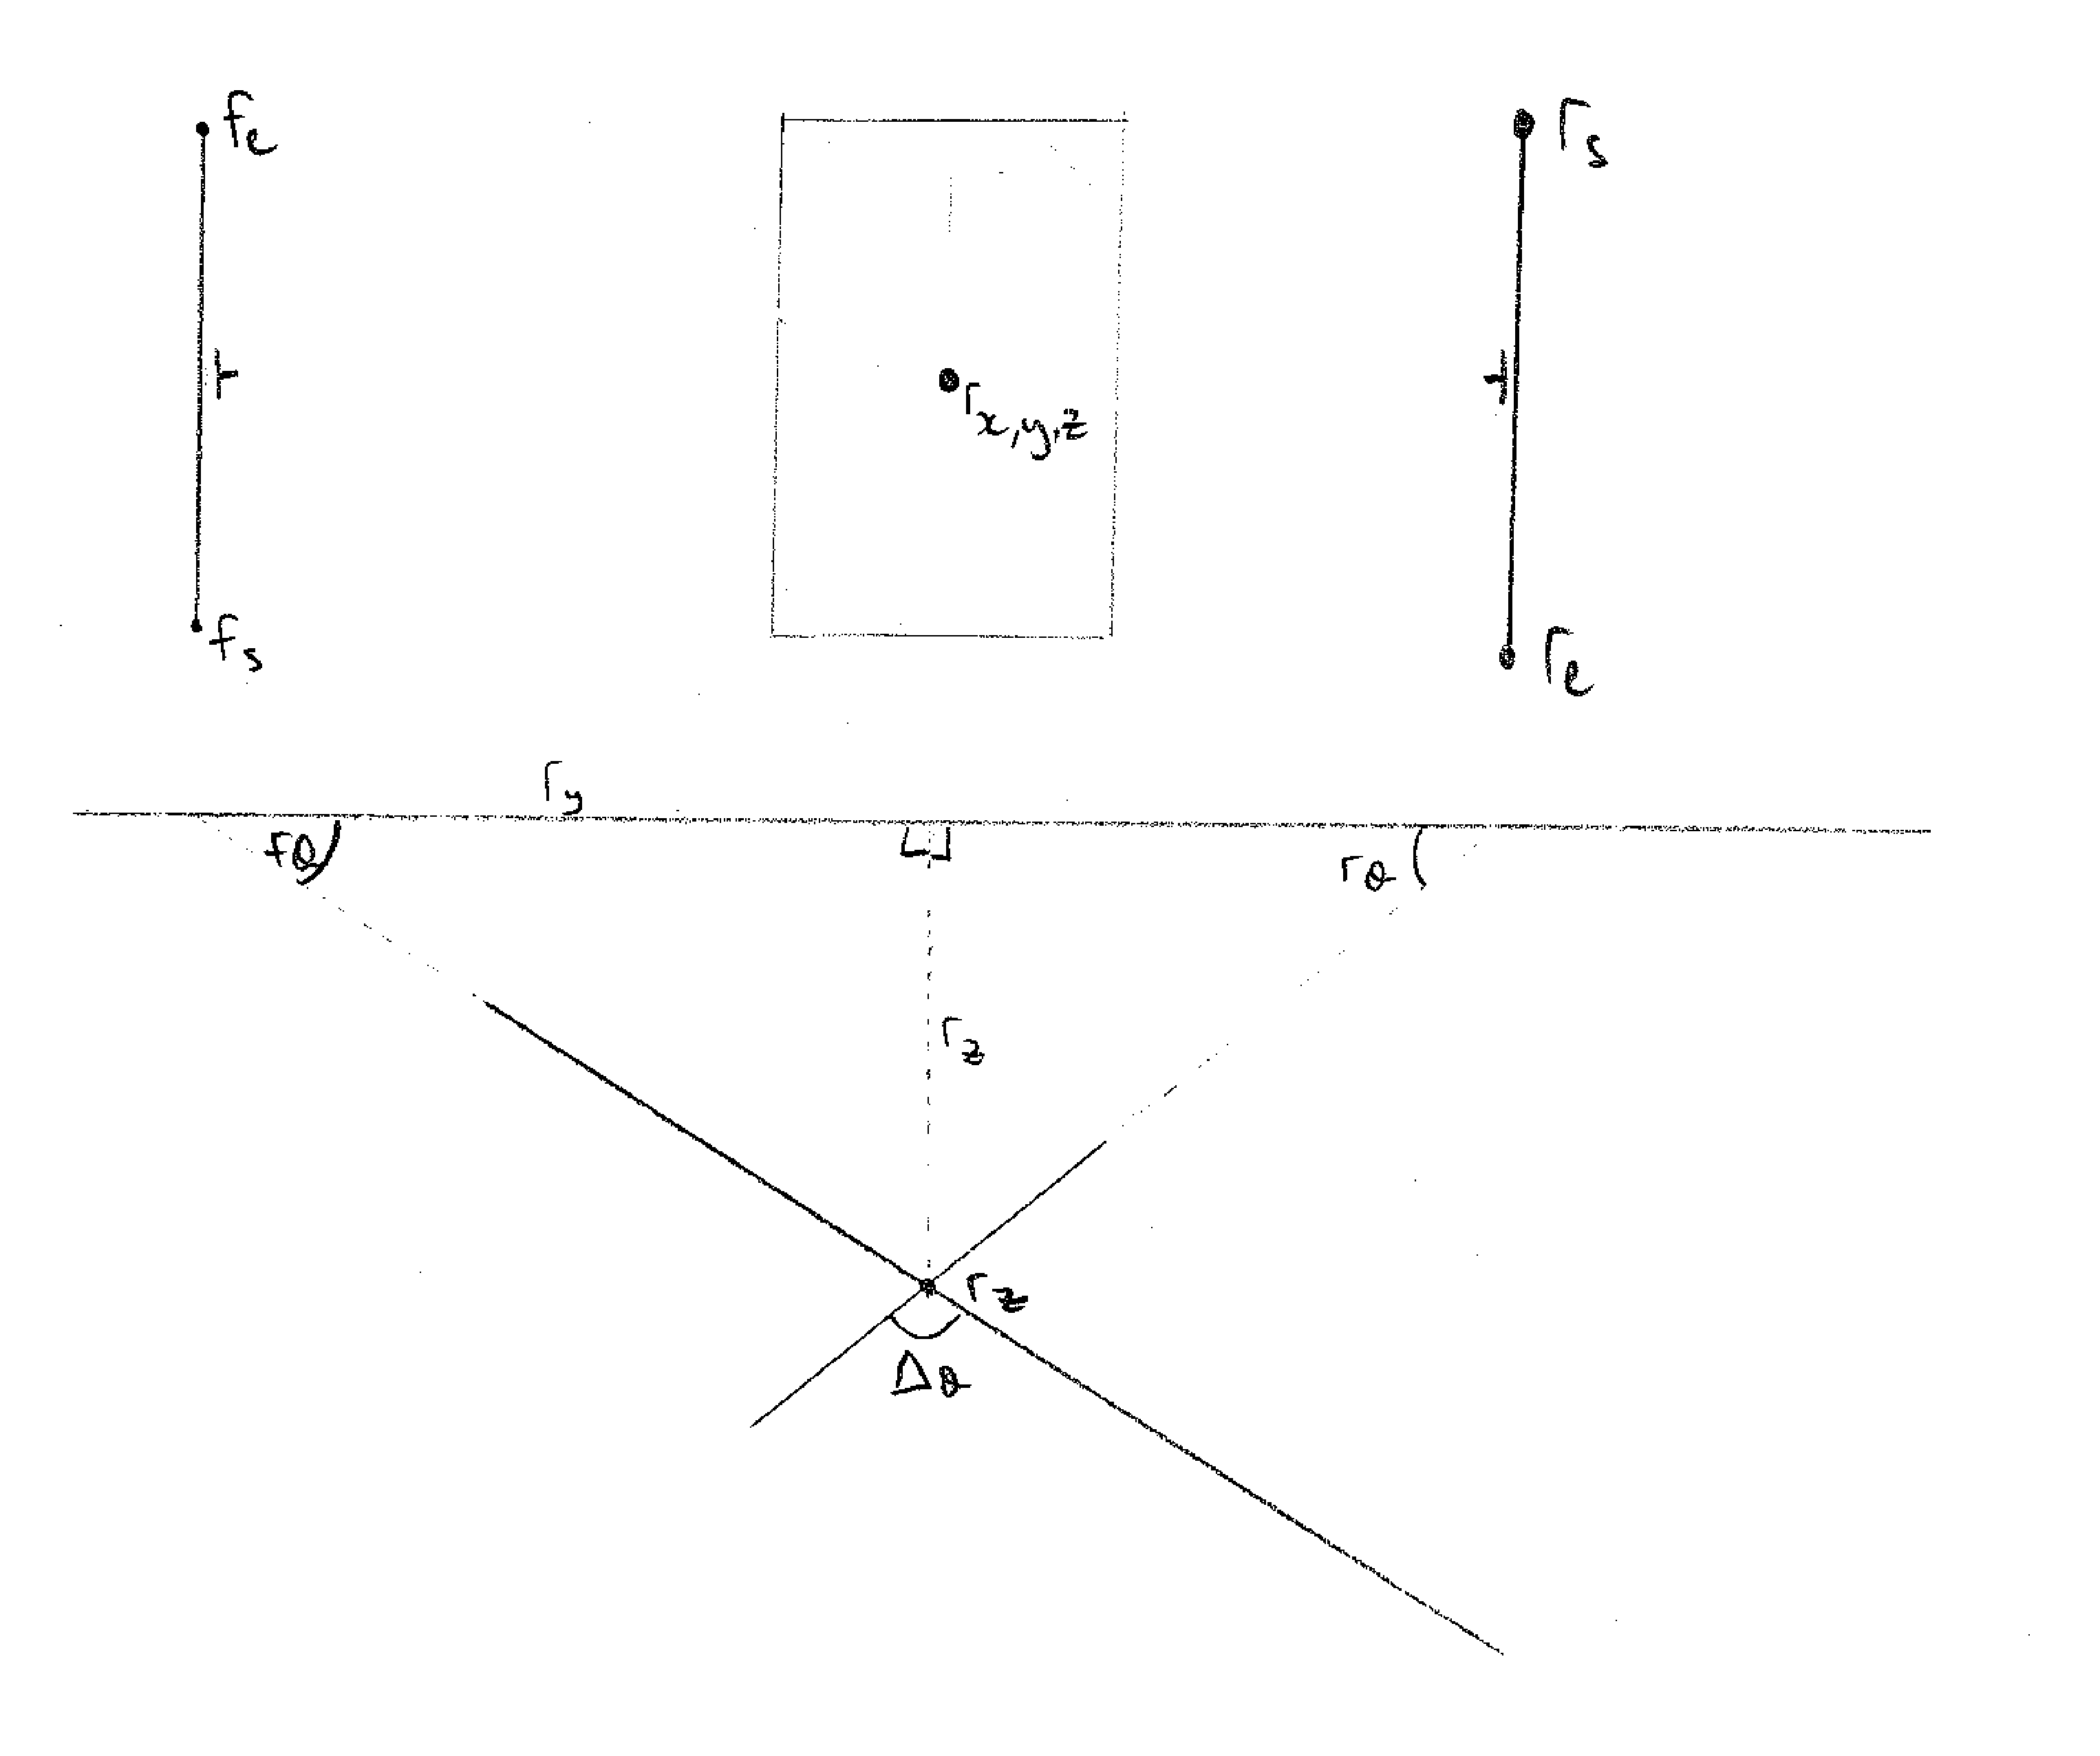
\includegraphics[width=14cm]
{gt90}}
\caption{Fault and rupture plane geometry for. Lower panel shows cross section view and upper panel shows a plan view of the surface 
projection. Note that in this case we need to re-project the rupture plane to the surface and redefine the start and end of the 
rupture trace such that the plane dips to the right hand side of the fault trace when looking from the start to end of the trace.}
\label{fig:gt90}
\end{figure}


We can follow the same approach as section \ref{sec:0to90} from equations \ref{rw090} to \ref{eq:rsx}. We need to slightly 
modify the next steps as we need to add instead of subtract $r_y$ to the right handside of the equation: 

\begin{equation}
\hat{r}_s^{y} = \hat{r}_y + r_z  \frac{cos(r_\theta * rad)}{sin(r_\theta * rad)}
\end{equation}

And now we can again follow the method in section \ref{sec:0to90} from equations \ref{eq:rex} to \ref{eq:rey}. 
But for equations \ref{eq:rsll} and \ref{eq:rell} we transform the coordinate system so the rupture start and end locations are swapped:

\begin{equation}\label{eq:rsll2}
r_e^{lon}, r_e^{lat } = \mathtt{azimuthal\_orthographic\_xy\_to\_ll}(\hat{r}_s^{x}, \hat{r}_s^{y}, \hat{r}_s^{lon},\hat{r}_s^{lat},f_\phi,\mbox{R}=6367.0)
\end{equation}

\begin{equation}\label{eq:rell2}
r_s^{lon}, r_s^{lat} = \mathtt{azimuthal\_orthographic\_xy\_to\_ll}(\hat{r}_e^{x}, \hat{r}_e^{y}, \hat{r}_s^{lon},\hat{r}_s^{lat},f_\phi,\mbox{R}=6367.0)
\end{equation}

Now we redefine the location of the rupture centroid in local x and y coordinates relative to the new 
origin ($r_s^{lon}$,$ r_s^{lat}$) of the new local coordinate system and then get the longitude and 
latitude of this point using equations \ref{eq:rx} to \ref{eq:rcll}.

%%%%%
\subsection{Case if  $180 <  r_\theta \leq f_\theta + \omega$} \label{sec:180to270}
%%%%%

If the initial $r_\theta$ value is greater than 180 but less than $f_\theta + \omega$ then the rupture 
plane dips in the same direction of the fault plane but the rupture trace lies behind the fault trace (figure \ref{fig:gt180}). 

Here we first obtain the dip of the rupture plane and force the dip to be greater than 5$^\circ$ so 
that the rupture trace projects to the surface:

\begin{equation}
r_\theta = \mathbf{max} \{ 180 - f_\theta + \omega, 5 \} .
\end{equation}

\begin{figure}[htp]
\centerline{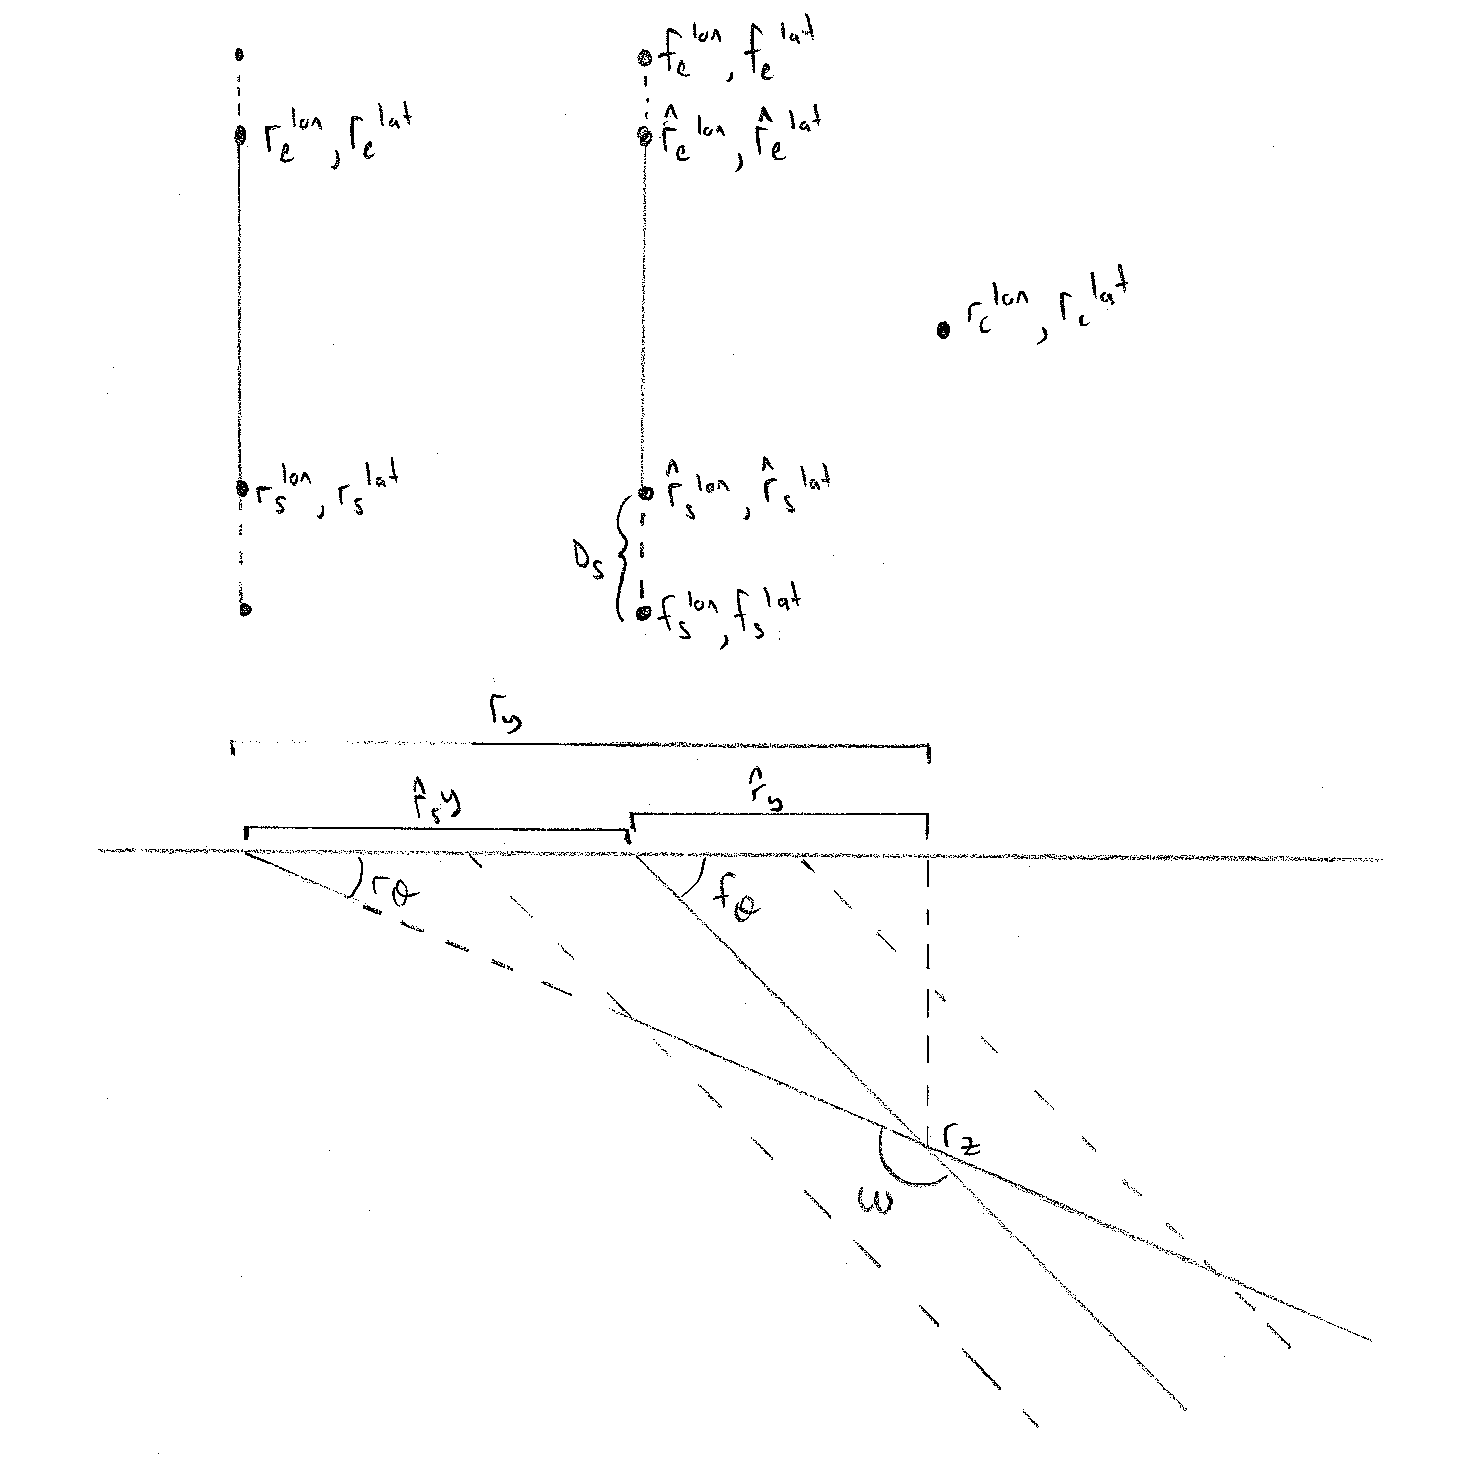
\includegraphics[width=14cm]
{gt180}}
\caption{Fault and rupture plane geometry for. Lower panel shows cross section view and upper panel shows 
a plan view of the surface projection. Note that in this case we need to re-project the rupture plane to 
the surface and redefine the start and end of the rupture trace.}
\label{fig:gt180}
\end{figure}

We follow the same methods as above up to equation \ref{eq:rsx} but now we change the following equation 
to solve for ($\hat{r}_y$) which in this case will be negative:

\begin{equation}\label{eq:ry4}
\hat{r}_s^y = \hat{r}_y -  r_z  \frac{cos(r_\theta  \times rad)}{sin(r_\theta \times rad)}.
\end{equation}

The end of the rupture trace in local coordinates ($\hat{r}_e^x$ and $\hat{r}_e^y$) referenced to the fault 
trace can be found from:
\begin{equation}
\hat{r}_e^x = r_l
\end{equation}

\begin{equation}
\hat{r}_e^y = \hat{r}_s^y
\end{equation}

Now we can follow equations \ref{eq:rsll} to \ref{eq:rcll} to get the remaining parameters.


\subsection{Overlapping source zones}

The concept of overlapping zones in a source model is useful for
accommodating background seismicity. In principle, the code can
accommodate overlapping seismic zones, i.e. where two seismic
zones share a common geographical region. However, it should be
noted that earthquakes will be distributed randomly in the common
region for each zone that exists. That is, a simulation using
overlapping source zones (such as that shown in
\fref{fig:h-source-overlapping}(a)) may lead to a greater number
of simulated earthquake\index{simulated earthquake}s in the common
region than may be warranted by the source model. This only poses
a problem if the recurrence relationship (i.e. the $a$, $b$
parameters) being used has not been modified to account for the
`double counting' in the simulated catalogue (generally this will
not have been done). To overcome this problem, it is advisable to
define the source zones in such a way that there are no
overlapping regions. \fref{fig:h-source-overlapping} demonstrates
two different techniques that can be used to incorporate
overlapping source zones in the EQRM. Both of the illustrated
techniques are based on creating a doughnut.

\begin{figure}[htp]
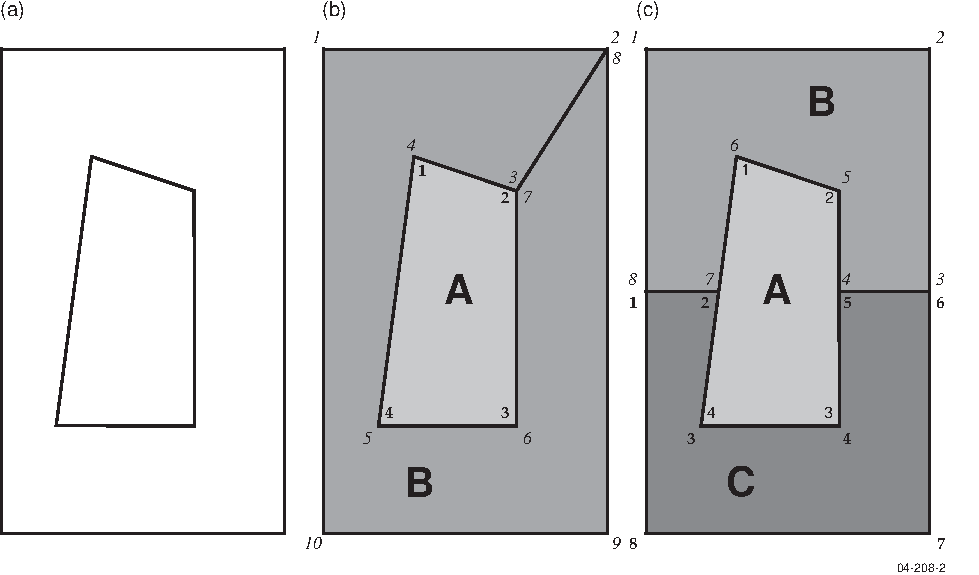
\includegraphics[width=1\textwidth]{fig-hsource-overlapping-zones}
\caption{Overlapping source zones shown in (a) can be incorporated
into the EQRM by cutting out a doughnut (b) or splitting the outer
polygon (c). The numbers in different fonts illustrate how the
polygon vertices could be listed in the
\typeparfilecaption{<site\_loc>}{\_par\_source}{zones}{.txt} file.
} \label{fig:h-source-overlapping}
\end{figure}



\subsection{Magnitude selection and event activity}
\label{sec:magnitude_selection}

A `stratified' Monte-Carlo technique is used to assign the event
magnitudes. The stratified nature of the technique ensures that
the full range of magnitudes is adequately sampled. The stratified
Monte-Carlo technique is illustrated in
\fref{fig-hattn-montecarlo} for the general case. This approach is
distinctly different to a brute force Monte-Carlo technique that
would preferentially sample the more probable lower magnitude
events. Such an approach would require the sampling of a large
number of small events to ensure that a handful of large events
are sampled.

The algorithm described in this section is the algorithm applied
when a single source model is used and the `generation
polygons'\index{generation polygon} are the source zones of the
source model. Some minor modifications are required when multiple
source models are used or the `generation
polygons'\index{generation polygon} differ from the source zones.
These modifications are described in \sref{sec:source-multizones}.


\begin{figure}[htp]
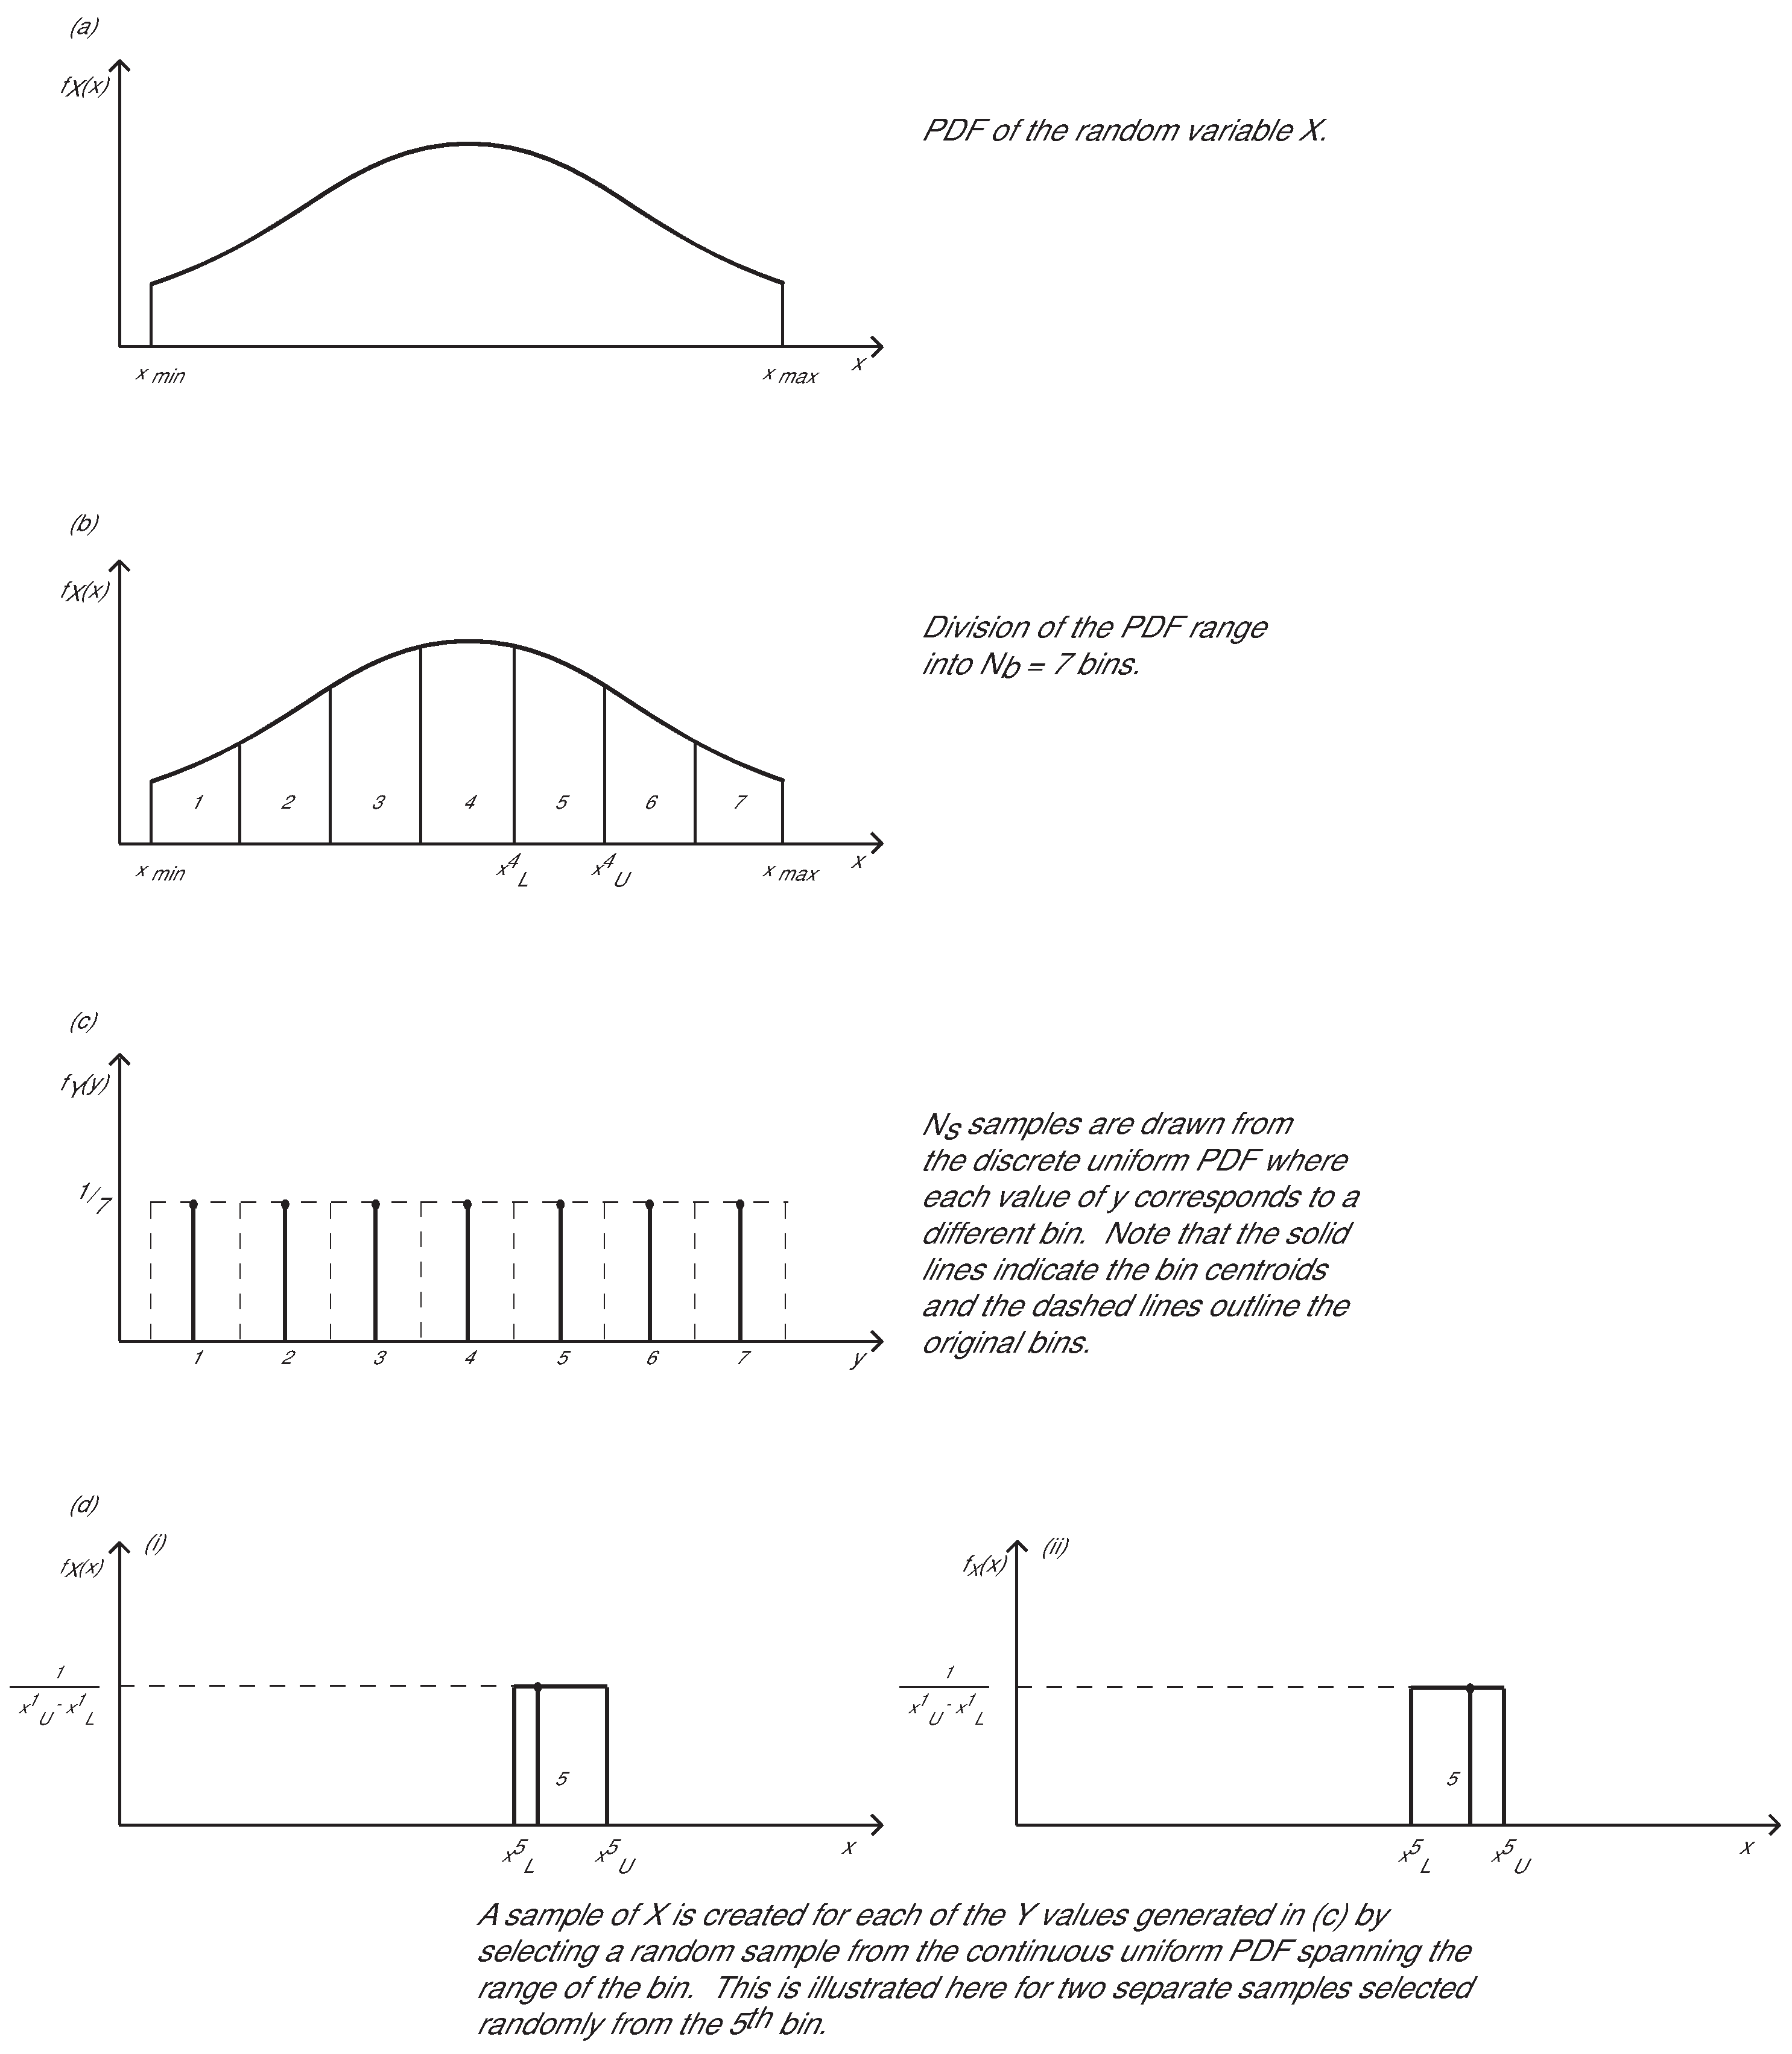
\includegraphics[width=1\textwidth]{fig-hattn-montecarlo}
\caption{Stratified Monte Carlo technique for sampling a PDF. In
this case a normal distribution is shown but any PDF can be used.}
\label{fig-hattn-montecarlo}
\end{figure}

The Probability Density Function (PDF) for the event magnitudes is
based on the bounded Gutenberg-Richter law \citep{dr_Kramer96a}.
The EQRM application simulates a number $N_s$ of earthquake
events. Considering the $i^{th}$ source zone, the algorithm for
choosing the magnitude of each event can be summarised as follows:

\begin{enumerate}
\item Bound the domain of the PDF with $m_{min}$ and $m_{max}$
(\fref{fig-hattn-montecarlo}a).

\item Separate the interval $[m_{min}, m_{max}]$ into $N_b$ bins,
and return the bin centroids (\fref{fig-hattn-montecarlo}b).

\item For each of the $N_{s,i}$ events randomly select a bin from
a discrete uniform
  distribution, where $N_{s,i}$ refers to the number of events in the $i^{th}$ source zone.
  This effectively leads to $N_{s,i}/N_b$ earthquakes in
  each magnitude bin and ensures that the full range of magnitudes
  is adequately sampled (\fref{fig-hattn-montecarlo}c).

\item For each of the $N_{s,i}$ events randomly select a magnitude
denoted $r_m$, from a
  continuous uniform distribution that spans the complete range of magnitudes in the
  bin. Note that Step 3 ensures that the entire range of magnitudes is
  adequately sampled whereas this step ensures that all magnitudes can be
  attained (\fref{fig-hattn-montecarlo}d).

\item For each of the $N_{s,i}$ events calculate the event
activity $r_\nu(r_m^*)$, where $r_m^*$ refers to the bin centroid
for the event in question and
\begin{equation}
\label{eq:event-activity} r_\nu(r_m^*) = \frac{N_b}{N_{s,i}}
\times \lambda(\typepar{min}{\_mag}{\_cutoff}) \times
P_{GR}(r_m^*-\Delta<R_m<r_m^*+\Delta).
\end{equation}
The first term in \eref{eq:event-activity}, $\frac{N_b}{N_{s,i}}$,
approximates the reciprocal of the number of synthetic events in
the bin. This term ensures that the event activity for each
synthetic event scales as the number of generated events is
modified and hence `brings the synthetic results back to the real
world'. The second term in \eref{eq:event-activity},
$\lambda(\typepar{min}{\_mag}{\_cutoff})$, represents the number
of earthquakes with magnitude greater than or equal to
\typepar{min}{\_mag}{\_cutoff} and is computed by evaluating the
bounded Gutenberg-Richter recurrence relation
\begin{equation}
\lambda(m) =
A_{min}\frac{e^{-\beta(m-m_{min})}-e^{-\beta(m_{max}-m_{min})}}{1-e^{-\beta(m_{max}-m_{min})}},
\end{equation}
\citep{dr_Kramer96a}. The final term in \eref{eq:event-activity}
represents the actual probability that a real event will fall into
the $r_m^*$ bin in a given year and is computed by evaluating
\begin{equation}
P_{GR}(r_m^*-\Delta<R_m<r_m^*+\Delta) =
\frac{f_M(r_m^*)}{\sum\limits_{j=1}^{N_b} f_M(r_{m,j}^*)}
\end{equation}
(\aref{app:discret-pdf}), where
\begin{equation}
f_M(r_m^*) = \frac{\beta
e^{-\beta(r_m^*-m_{min})}}{1-e^{-\beta(m_{max}-m_{min})}},
\end{equation}

\begin{equation}
\beta = b\ln(10)
\end{equation}
\citep{dr_Kramer96a} and $\Delta$ is the half width of the bins.
Note that $r_\nu$ represents the frequency of occurence in terms
of a number per year and can be thought of as the synthetic
version of $\lambda$ for the simulated event catalogue.
\end{enumerate}

\Frefmulti{fig:source-catalogue-results1}{fig:source-catalogue-results3}(a)
illustrate histograms of the event magnitudes simulated for three
different source zone combinations. Note that the fifteen bars in
\Freftwo{fig:source-catalogue-results1}{fig:source-catalogue-results2}(a)
correspond to the fifteen different magnitude bins. The event
activity $r_v$ for the same source zone combinations are shown in
\Frefmulti{fig:source-catalogue-results1}{fig:source-catalogue-results3}(c).

\begin{figure}
  \vspace{0.8em}
\begin{center}
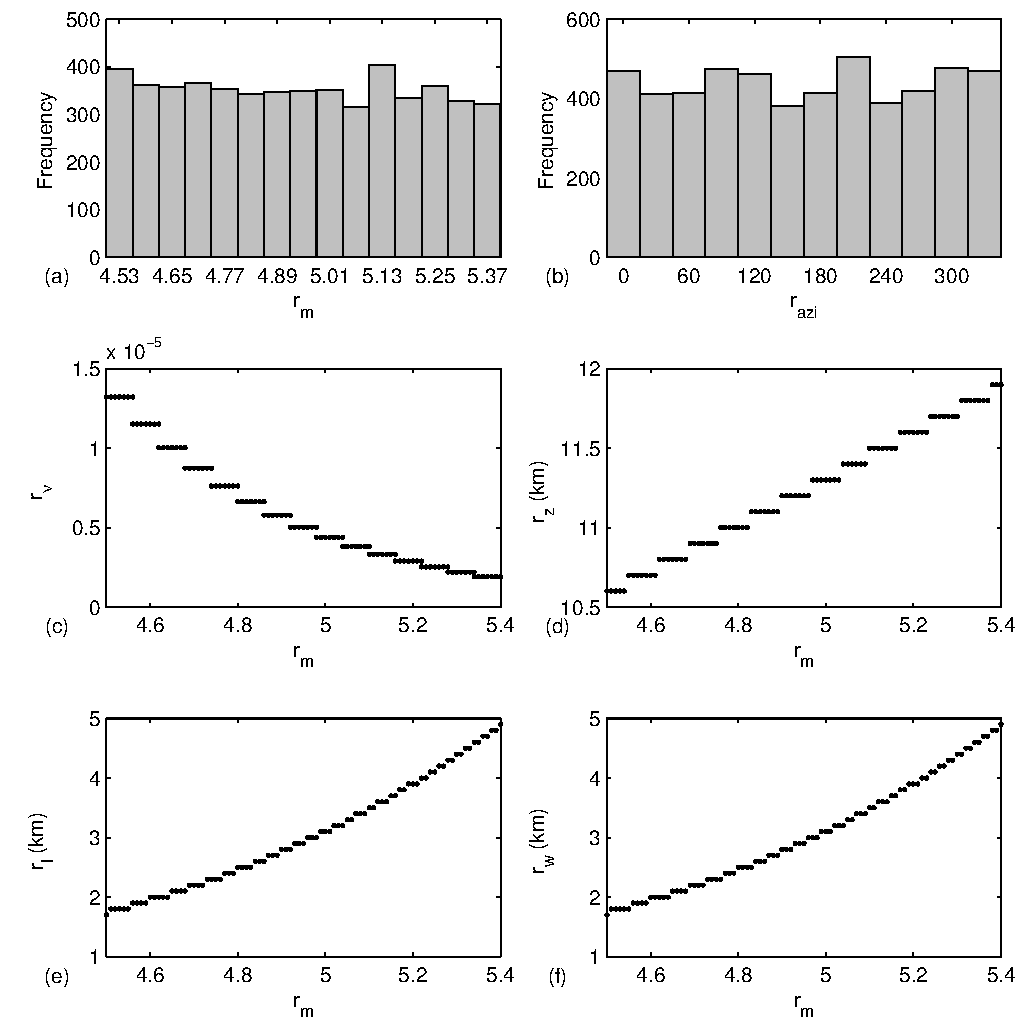
\includegraphics[width=1\textwidth]{fig-hsource-eventstatstri}
\end{center}
\caption{Simulated events for the Newcastle Triangle Zone (see
\citealt{dr_Dhu02b}). Plots (a) and (b) show histograms of the
rupture magnitude $r_m$ and rupture azimuth $r_{azi}$
respectively. Plots (c), (d), (e) and (f) illustrate the
relationship between the event magnitude $r_m$ and the event
activity $r_\nu$, the depth to the rupture centroid $r_z$, the
length of the rupture $r_l$ and the width of the rupture $r_w$
respectively. The desired number of events $ntrgvector(1)$ was
$5000$.} \label{fig:source-catalogue-results1}
\end{figure}

\begin{figure}
\begin{center}
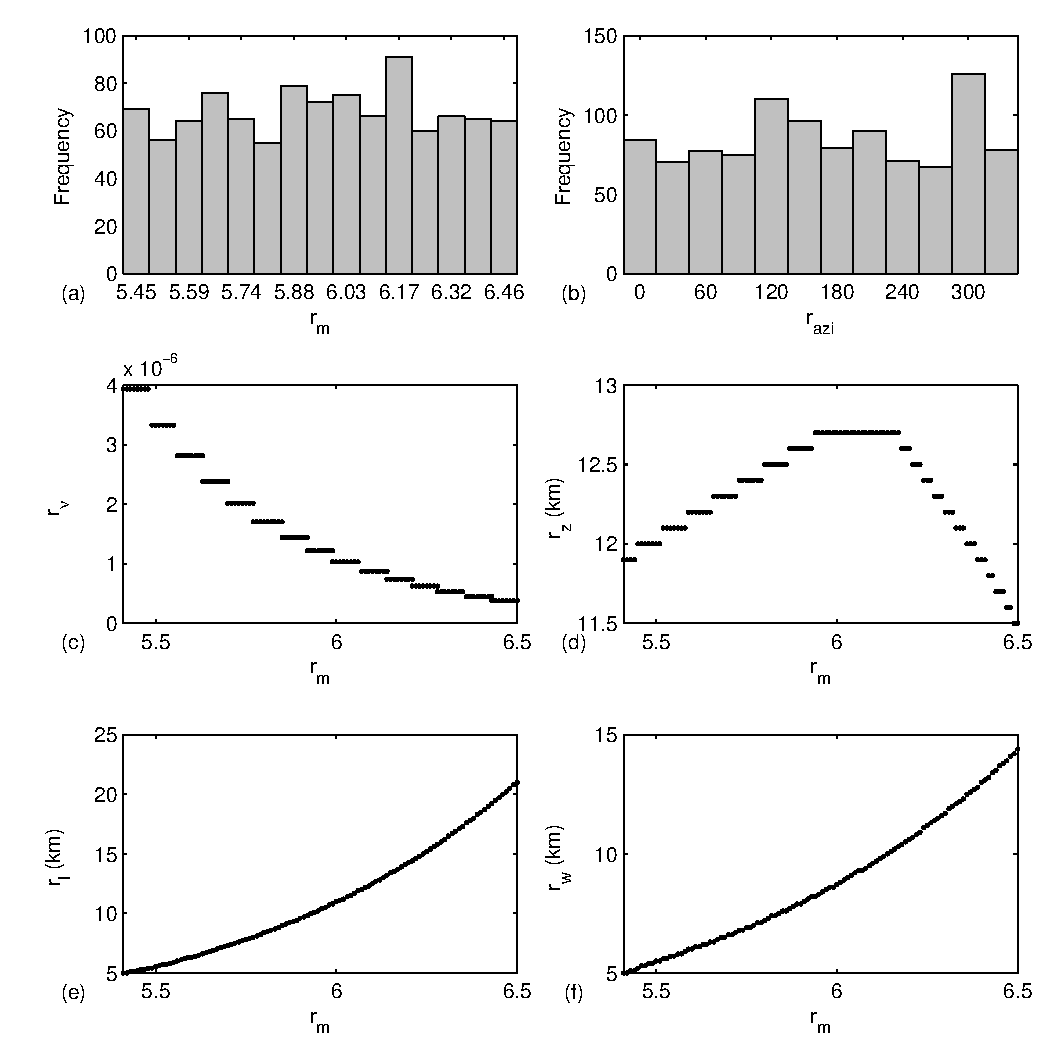
\includegraphics[width=1\textwidth]{fig-hsource-eventstatsrec}
\end{center}
\caption{Simulated events for the Newcastle Rectangle Zone (see
\citealt{dr_Dhu02b}). Parts (a) to (f) are the same as those
described in \fref{fig:source-catalogue-results1}. The desired
number of events $ntrgvector(4)$ was $3000$.}
\label{fig:source-catalogue-results2}
\end{figure}

\begin{figure}
\begin{center}
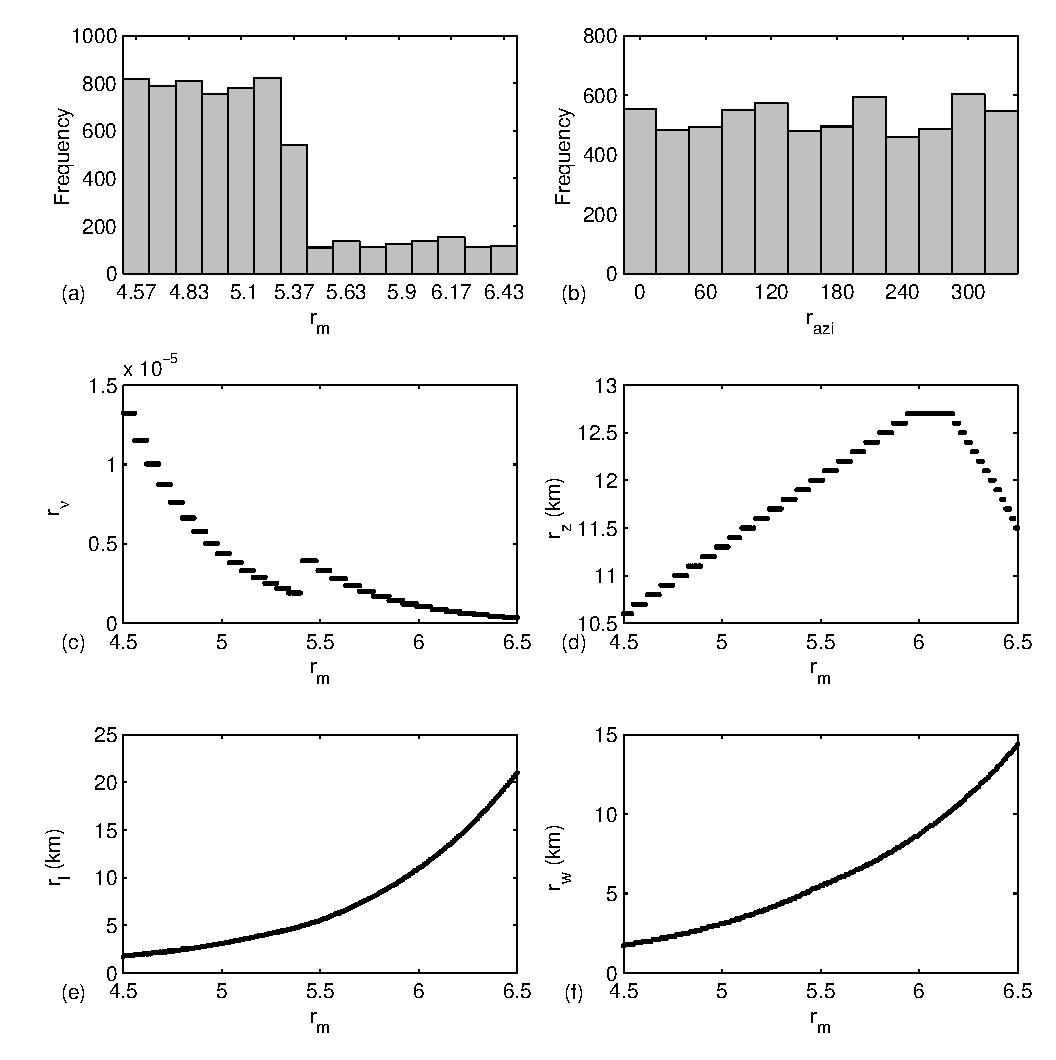
\includegraphics[width=1\textwidth]{fig-hsource-eventstats_tri_rec}
\end{center}
 \caption{Simulated
events when the Newcastle Triangle Zone and Newcastle Fault Zone
are considered together (see \citealt{dr_Dhu02b}). Parts (a) to
(f) are the same as those described in
\fref{fig:source-catalogue-results1}. The desired number of events
was defined by $ntrgvector = [5000,3000]$ where the source zones
$1$ and $2$ refer to the the Newcastle Triangle Zone (NTZ) and the
Newcastle Fault Zone respectively.}
\label{fig:source-catalogue-results3}
\end{figure}



\begin{figure}
\begin{center}
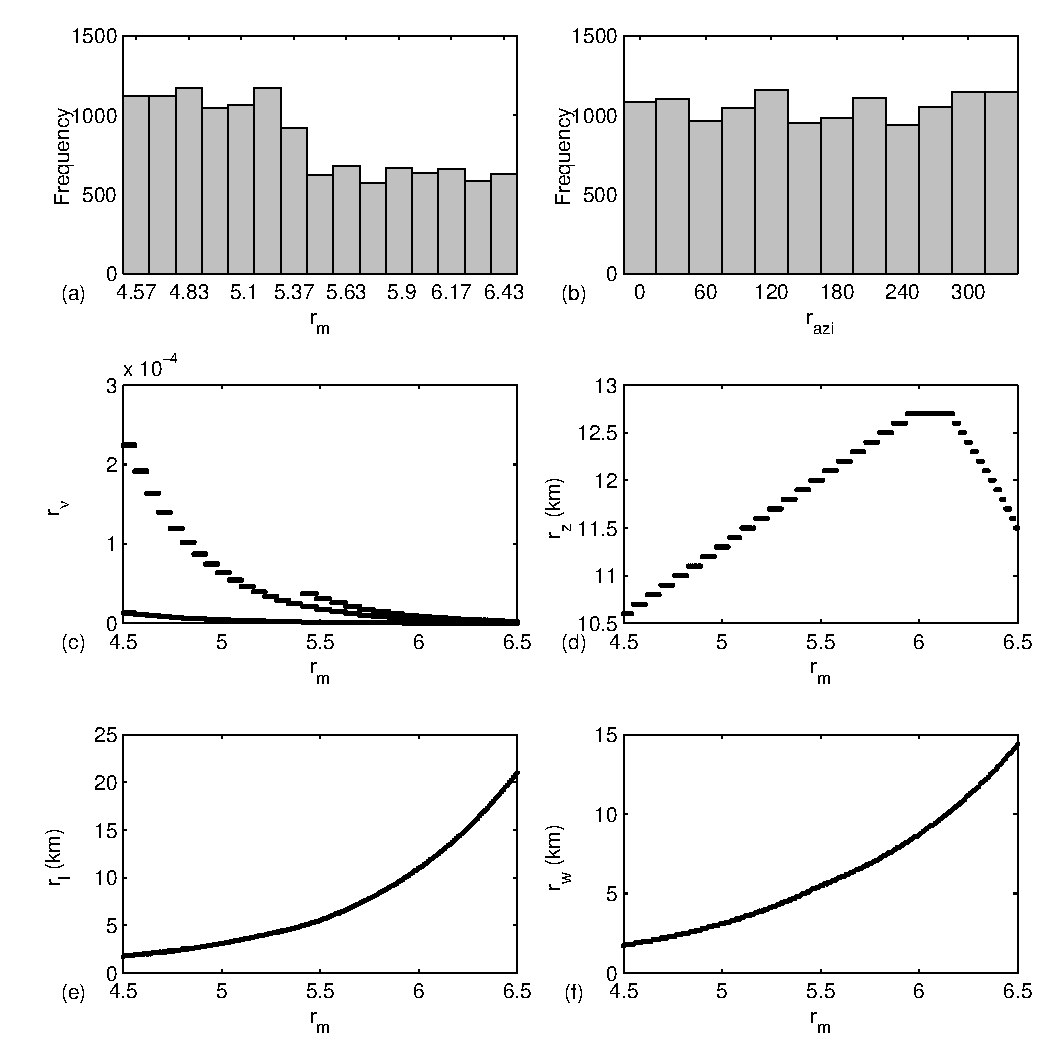
\includegraphics[width=1\textwidth]{fig-hsource-eventstatsall}
\end{center}
\caption{Simulated events for all six of the source zones used in
the Newcastle and Lake Macquarie study (see \citealt{dr_Dhu02b}).
Parts (a) to (f) are the same as those described in
\fref{fig:source-catalogue-results1}. The desired number of events
was defined by $ntrgvector = [5000,1000,1000,3000,1000,1000]$
where the source zones $1$ to $6$ refer to the the Newcastle
Triangle Zone (NTZ) the Tasman Sea Margin Zone Subset 1 (TSMZ1),
the TSMZ2, the Newcastle Fault Zone, the TSMZ3 and the TSMZ4
respectively.} \label{fig:source-catalogue-results4}
\end{figure}


\subsection{Dimensions and position of the rupture plane}
\label{sec:dim-rupture}


The width and length of the rupture and position of the rupture
centroid are computed by \typefunc{mag}{2rup}{\_v} using empirical
rules based on the moment magnitude, $r_m$ of the event (Mendez,
2002 [\textit{pers. comm.}]) . The location of the rupture plane
is constrained to lie within a virtual fault\index{virtual fault}
which is described by the depth to its top (equivalent to the
depth to the seismogenic region $f_z$, see
\sref{tab:site-loc-par-sourcezones}), its length $f_l$, its width
$f_w$ and its dip $r_{dip}$. Note that by default the dip of the
 rupture plane is defined to be the dip of the virtual fault\index{virtual fault}.
Firstly, the area of the rupture plane $A_r$ is defined as
\begin{equation}
A_r = 10^{r_m - 4.02}
\end{equation}
which represents a subtle change from that defined by
\citet*{dr_Wells94a}. Empirical relationships for the width $r_w$
and length $l_r$ of the rupture plane were defined by Mendez (2002
[\textit{pers. comm.}]). The width is defined in a two step
process as follows
\begin{equation}
 f_1 = \left \{ \begin{array}{ll}
 1 & \textrm{if $r_m \leq 5.5$} \\
\frac{1}{\sqrt[\leftroot{-2}\uproot{2}4]{1+2(r_m-5.5)\sin(r_{dip})}} & \textrm{if $r_m>5.5$} \\
\end{array} \right.
\end{equation}

and

\begin{equation}
r_w = \textrm{min$\{f_1\sqrt{A_r},f_w\}$}.
\end{equation}

Recall from \sref{sec:event-catalogue} that the rupture centroid
$(r_x,r_y,r_z)$ is defined in terms of a local coordinate system.
The depth of the rupture centroid is determined in a two step
process as follows:

\begin{equation}
f_2 = \left \{ \begin{array}{ll} 1 & \textrm{if $r_m\leq4$} \\
1 + \frac{r_m-4}{2} & \textrm{if $4<r_m\leq6$} \\
2 & \textrm{if $r_m\geq6$} \\
\end{array} \right.
\end{equation}

and
\begin{equation}
r_z = \textrm{min$\{f_z+\frac{f_2}{3}f_w\sin(r_{dip}),
f_z+f_w\sin(r_{dip})-\frac{1}{2}r_w\sin(r_{dip})\}$}.
\end{equation}

The other two coordinates of the rupture centroid are given by
\begin{equation}
r_y = r_z\cot(r_{dip})
\end{equation}

and

\begin{equation}
r_x = \frac{r_l}{2}.
\end{equation}
The depth to the rupture centroid $r_z$ and the length and width
of the rupture plane are illustrated for four separate simulations
in
\Frefmulti{fig:source-catalogue-results1}{fig:source-catalogue-results4}(d),
(e) and (f) respectively.



\subsection{Azimuth and dip of rupture}
\label{sec:az-dip-rupture}

The rupture azimuth of each event may be forced to lie within a
user defined range
\begin{center} $\phi - d_{\phi} \leq r_\phi \leq \phi + d_{\phi}$ \end{center}
where $\phi$ and $d_{\phi}$ are \typepar{a}{z}{i} and
\typepar{d}{\_a}{zi} in \typeself{set}{da}{ta} respectively. The
default values for $\phi$ and $d_{\phi}$ are $180^o$ and $180^o$
respectively. Recall that the azimuth is further adjusted through
the process described in \sref{sec:rup-location}, unless $d_{azi}$
is assigned to a negative number. Note that in the current version
of the EQRM application this adjustment process ignores the above
azimuth bound. That is, the azimuth of one or more events may be
adjusted outside the above range in an attempt to force the
event's end point to lie within the source zone. The distribution
of simulated azimuth for four different simulations is illustrated
in
\Frefmulti{fig:source-catalogue-results1}{fig:source-catalogue-results4}(b).

The dip of the rupture, $r_{dip}$, is assigned in
\typeself{set}{da}{ta} and may take only a single value for all
source zones. The dip of the rupture trace is measured from the
ground surface and the direction of dip is such that the plane is
located in the region of $y>0$ in the local coordinate system.
Note that it is
 possible to modify the software to select the dip randomly in a similar fashion to that
 described for the azimuth above. However, it is worth noting that
 the effect of a change in dip varies based on the attenuation model (see \sref{ch:atten}). For example, when using an attenuation model that depends on the Joyner-Boore distance, the practical effect
 of a change in dip can be compensated by a
 horizontal translation of the rupture trace. In such cases the random
 location of the rupture trace negates the need to select the dip
 randomly.

\section{Using multiple source zones - Incorporating epistemic uncertainty}
\label{sec:source-multizones}

Recall that \sref{sec:source-EQcat} introduced two techniques for
passing source models to the EQRM:
\begin{enumerate}
\item the
\typeparfilecaption{<site\_loc>}{\_par}{\_sourcezones}{.txt} and
\typeparfile{<site\_loc>}{\_par\_sou}{rcepolys}{.txt} file pair,
and \item the
\typeparfilecaption{<site\_loc>}{\_par}{\_source}{.mat} file.
\end{enumerate}
Recall also that the notion of a `generation
polygon'\index{generation polygon} was introduced where the
generation polygons are simply the individual source zones when
Technique 1 is used, and `generation polygon' refers to the
polygons in the \typevar{gen}{erat}{ion} variable when Technique 2
is used. This definition ensured that the discussion of earthquake
location (\sref{sec:rup-location}), rupture geometry
(\sref{sec:dim-rupture}), azimuth and dip
(\sref{sec:az-dip-rupture}) described above is applicable to both
of the two techniques for providing source information to the
EQRM. When Technique 2 is used, however, a minor modification must
be made to the algorithm described for magnitude and event
activity determination (see \sref{sec:magnitude_selection}). To
explain the differences in the algorithm and to explain the
incorporation of multiple source zone models (epistemic
uncertainty with source models) the reader will need to understand
the contents of the
\typeparfile{<site\_loc>}{\_par}{\_source}{.mat} file.

The \typeparfile{<site\_loc>}{\_par}{\_source}{.mat} file contains
the following two variables:
\begin{enumerate}
\item The \typevar{gen}{erat}{ion} variable is a MATLAB structure
containing the fields \texttt{zones} and \texttt{polys}. The field
\texttt{zones} is a matrix containing the same format as that
described in \tref{tab:site-loc-par-sourcezones}. The number of
rows refers to the number of `generation polygons' to be used in
the generation process. It is common to have 2 `generation
polygons' arranged in a doughnut shape with an inner and outer
polygon. The inner polygon is typically centered on the region of
interest and can be used to simulate a larger number of
earthquakes (hence higher spatial concentration) than the outer
polygon. The field \texttt{polys} is a matrix using the same
format as \tref{tab:site-loc-par-sourcepolys} to describe the
vertices of the polygons in the field \texttt{zones}. \item The
\typevar{sou}{rc}{e} variable is a MATLAB structure array
containing one element for each source zone model to be used. The
number of elements in the \typevar{sou}{rc}{e} structure array
corresponds to the number of source zone models to be used in the
simulation. Each element has fields \texttt{zones}, \texttt{polys}
and \texttt{weight}. The fields \texttt{zones} and \texttt{polys}
are similar to those described in 1 above, however this time they
represent the individual source source zones for the source model.
The field \texttt{weight} represents the weight to be applied to
the source zone model.
\end{enumerate}

When using Technique 2 the \typevar{gen}{er}{ation} is used to
define the `generation polygons' and hence the location, geometry,
azimuth and dip of the rupture. The variable
\typevar{gen}{er}{ation} is also used to assign magnitudes to each
synthetic event\index{synthetic event} using Steps 1 to 4 from
\sref{sec:magnitude_selection}. Note that a synthetic earthquake
generated in this fashion may lie in none, one or multiple source
zones from the different source models. The calculation of an
event activity involves identifying which zones the earthquake
lies within and then computing the weighted sum of individual
event activities for the zones within which it lies. The algorithm
for computing the event activity for a single source zone is
described in Step 5 of \sref{sec:magnitude_selection}. Note that
an earthquake must fall within the polygon that defines the source
zone and its magnitude must be within the magnitude bounds for the
source zone before it is considered to lie within the source zone.
More details of this process can be found by looking at the
functions \typefunc{calc}{\_event}{\_activity} for the calculation
of event activity and \typefunc{mke}{\_aseq}{4mat} for all of
processes.

\section{Spawning events}
\label{source:spawning}


There is an option within the EQRM application to spawn (or copy)
events. Such copies are required by some techniques for
incorporating aleatory uncertainty in later stages of the PSHA and
PSRA. For example, \sref{attn:uncert-randomchoice} describes an
incorporation of aleatory attenuation uncertainty that does not
require spawning of the catalogue whereas
\sref{attn:uncert-pdfchoice} describes a process that does require
spawning.  The option is performed by \typefunc{fuse}{\_4}{hzd}.
Actually \typefunc{fuse}{\_4}{hzd} is an essential component of
any earthquake hazard or risk run with the
\typeselfnoindex{}{}{EQRM} application i.e. it must be run
regardless of whether the user wishes to spawn events or not. The
spawning of events is controlled by \typepar{src}{\_eps}{\_switch}
in \typeself{set}{da}{ta}. If
\mbox{\typepar{src}{\_eps}{\_switch}$ = 1$ or $-1$} then all
events with magnitude greater than $m_{bnd}$ (\typepar{m}{bn}{d}
in \typeself{set}{da}{ta}) are copied $n_{samples}$
(\typepar{nsa}{mpl}{es} in \typeself{set}{da}{ta}) times with
their event activity adjusted according to a weight $w_e$. If
\mbox{\typepar{src}{\_eps}{\_switch}$ = 0$} no spawning is
undertaken. When spawning the weight $w_e$ is derived by
truncating and re-normalising a standard normal distribution to
$\pm n_\sigma$ (\typepar{n}{sig}{ma} in \typeself{set}{da}{ta}).
The process is summarised below.

We know that the standard normal distribution $ N \sim (0,1)$ has
a PDF given by
\begin{equation}
\begin{array}{lr}
f_X(x)=\frac{1}{\sqrt{2\pi}}e^{\frac{-x^2}{2}} & - \infty <x<
\infty.
\\
\end{array}
\end{equation}

To truncate and re-normalise $N \sim (0,1)$ to $\pm n_\sigma$ we
must evaluate $P(-n_\sigma \sigma \leq X \leq n_\sigma \sigma)$.
The error function
\begin{equation}
erf(x) = \frac{2}{\sqrt{\pi}} \int_{0}^{x} e^{-t^2} \, dt.
\end{equation}
is related to the cumulative area under the standard normal
distribution via
\begin{equation}
erf(x) = 2P(X \leq x)-1.
\end{equation}
The function \typefunc{mke}{\_ct}{pdf} computes $P(-n_\sigma
\sigma \leq X \leq n_\sigma \sigma)$ using the error function as
follows
\begin{equation}
\begin{array}{rcl}
P(-n_\sigma \sigma \leq X \leq n_\sigma\ \sigma)  & = & P(X \leq
n_\sigma)-P(X \leq -n_\sigma) \\
   & = & 2P(X \leq n_\sigma)-1 \\
    & = & erf(n_\sigma) . \\
\end{array}
\end{equation}

Then, \typefunc{mke}{\_ct}{pdf} computes the truncated and
re-normalised PDF by evaluating
\begin{equation}
\begin{array}{lr}
\tilde{f}_X(x)= \frac{1}{P(-n_\sigma \sigma \leq X \leq n_\sigma
\sigma)}
\frac{1}{\sqrt{2\pi}}e^{ \frac{-x^2}{2}} & -n_\sigma \sigma <x< n_\sigma \sigma. \\
\end{array}
\end{equation}

The observant reader will notice that because the EQRM application
works in the discrete world, simply evaluating $\tilde{f}_X(x)$
will not suffice. The approach used by \typefunc{mke}{\_ct}{pdf}
to discretise $\tilde{f}_X$ and compute the weights
$\{w_{e,i}\}_{i=1}^{n_{samples}}$ is identical to that used to
compute the event activity $r_\nu$ (see
\sref{sec:magnitude_selection}) and is described in
\aref{app:discret-pdf}. That is
\begin{equation}
w_{e,i} = \frac{\tilde{f}_X(x_i)}{\sum\limits_{j=1}^{n_{samples}}
\tilde{f}_X(x_j)}.
\end{equation}
Once the weights $\{w_{e,i}\}_{i=1}^{n_{samples}}$ are computed
the event activity $r_\nu$ for each of the event copies is
re-defined as follows:
\begin{equation}
\label{source:spawning-activity}
\begin{array}{ll}
r_{\nu,i} = r_{\nu,original} \times w_{e,i} & \textrm{for } i=1
\textrm{ to } n_{samples},
\end{array}
\end{equation}
for each copy of the original event and its associated weighting.
A source epsilon term $r_\varepsilon$ is also defined for each
copy of the original event i.e.
$\{r_{\varepsilon,i}\}_{i=1}^{n_{samples}}$. Each of the
$r_{\varepsilon,i}$ are defined such that they correspond to the
$i^{th}$ bin centroid from the $n_{samples}$ bin spanning $\pm
n_\sigma$ (see \sref{attn:uncert-pdfchoice} for the mathematical
definition).


\section{Analysing a scenario event}
\label{sec:source-scenario} The EQRM application (through
\typefunc{mke}{\_ev}{nts}) incorporates an option for considering
a particular (or scenario) event. This option is instigated when
the user defines \typepar{det}{erm}{\_flag}$=1$ in
\typeself{set}{da}{ta}. The earthquake catalogue takes the same
form as that described in \tref{tab:evntdb-columns}. The scenario
event is constrained by user defined values for magnitude
(\typepar{det}{erm}{\_mag}), position
(\typeparcaption{det}{erm}{\_lat} and \typepar{det}{erm}{\_lon}),
depth (\typeparcaption{det}{erm}{\_r\_z}) and azimuth
(\typepar{det}{erm}{\_azi}).

\newpage
\section{Key functions, flags and parameters}

\begin{tabular}{llp{0.55\textwidth}}
\hline
\textbf{Name} & \textbf{Type} & \textbf{Description} \\
\hline
\keyrowsep \typefunc{mke}{\_ev}{nts} & Function & Master file for creating an event catalogue.\\
\keyrowsep \typefunc{mke}{\_aseq}{4mat} & Function & Handles a significant proportion of the synthetic event generation on behalf of \typefunc{mke}{\_ev}{nts}. \\
\keyrowsep \typefunc{m2}{gr}{pdfb} & Function & Computes the PDF, $f_M$ for the bounded Gutenberg-Richter distribution. \\
\keyrowsep \typefunc{mag}{2rup}{\_v} & Function & Computes rupture dimension and `relative' location based on magnitude. \\
\keyrowsep \typefunc{fuse}{\_4}{hzd} & Function & Master file for spawning events. \\
\keyrowsep \typefunc{mke}{\_ct}{pdf} & Function & Truncates and discretises $N\sim(0,1)$. \\
\keyrowsep \typepar{a}{z}{i} & Par & Centre of azimuth range for events. \\
\keyrowsep \typepar{d}{\_a}{zi} & Par & Half width of azimuth range. \\
\keyrowsep \typepar{d}{i}{p} & Par & Dip of virtual fault\index{virtual fault}. \\
\keyrowsep \typepar{ntrg}{vec}{tor} & Par & Vector whose elements represent the desired number of events to be simulated in each source zone. \\
\keyrowsep \typepar{w}{d}{th} & Par & Width of virtual fault\index{virtual fault}. \\
\keyrowsep \typepar{n}{bin}{s} & Par & Number of bins for event magnitude sampling. \\
\keyrowsep \typepar{src}{\_eps}{\_switch} & Par &  Events are (not) spawned if \typepar{src}{\_eps}{\_switch} $= 1$ ($=0$). \\
\keyrowsep \typepar{m}{bn}{d} & Par &  Only events with magnitude greater than \typepar{m}{bn}{d} are spawned. \\
\keyrowsep \typepar{nsa}{mpl}{es} & Par & Creates \typepar{nsa}{mpl}{es} copies of each spawned event. \\
\keyrowsep \typepar{n}{sig}{ma} & Par &  Range of distribution to be considered when spawning. \\
\keyrowsep \typepar{det}{erm}{\_flag} & Par & EQRM application used in scenario mode if \typepar{det}{erm}{\_flag} $=1$. \\
\keyrowsep \typepar{det}{erm}{\_mag} & Par & Magnitude of scenario event. \\
\end{tabular}


\begin{tabular}{llp{0.55\textwidth}}
\keyrowsep \typepar{det}{erm}{\_lat} & Par & Latitude of scenario epicenter (corresponds to $r_c^{lat}$). \\
\keyrowsep \typepar{det}{erm}{\_lon} & Par &  Longitude of scenario epicenter (corresponds to $r_c^{lon}$). \\
\keyrowsep \typepar{det}{erm}{\_r\_z} & Par &  Depth to scenario epicenter in $km$ (corresponds to $r_z$). \\
\keyrowsep \typepar{det}{erm}{\_azi} & Par &  Azimuth of scenario event (corresponds to $r_\phi$). \\
\hline
\end{tabular}






%%% Local Variables:
%%% mode: latex
%%% TeX-master: "eqrmtech"
%%% End:
